% Capitolul 13: Bule speculative: modele LPPL
% Serii de timp -- Programele de licență Informatică economică și Cibernetică economică, Academia de Studii Economice din București
% GENERAT de latex/build_chapter13.py -- modificați generatorul, nu acest fișier.

\newcommand{\coursename}{Serii de timp}
\def\tsalang{ro}
% Preambul comun TSA -- Serii de timp / Time Series Analysis (Beamer, 16:9)
% Același design ca MFM și SFM (preluat din SFM, 5 octombrie 2026). Înainte de % Preambul comun TSA -- Serii de timp / Time Series Analysis (Beamer, 16:9)
% Același design ca MFM și SFM (preluat din SFM, 5 octombrie 2026). Înainte de % Preambul comun TSA -- Serii de timp / Time Series Analysis (Beamer, 16:9)
% Același design ca MFM și SFM (preluat din SFM, 5 octombrie 2026). Înainte de \input{../../latex/preamble} se definește
%   \newcommand{\coursename}{Time Series Analysis}      (EN)
%   \newcommand{\coursename}{Serii de timp}       (RO)  și  \def\tsalang{ro}
% Fișierele .tex se află în EN/Courses, EN/Seminars, RO/Cursuri, RO/Seminarii (două niveluri sub rădăcină).
% Deck-urile sînt generate de latex/build_chapterN.py / build_seminarN.py (vezi latex/tsa_build.py).

\documentclass[9pt, aspectratio=169, t]{beamer}
\providecommand{\coursename}{Time Series Analysis}

% Ensure content fits on slides
\setbeamersize{text margin left=8mm, text margin right=8mm}
% Smaller institute font (title page)
\setbeamerfont{institute}{size=\footnotesize}

%=============================================================================
% THEME AND STYLE CONFIGURATION
%=============================================================================
\usetheme{default}
% Using default theme for clean header/footer control

% Color Palette (matching Redispatch PDF)
\definecolor{MainBlue}{RGB}{26, 58, 110}
\definecolor{AccentBlue}{RGB}{26, 58, 110}
\definecolor{IDAred}{RGB}{205, 0, 0}
\definecolor{DarkGray}{RGB}{51, 51, 51}
\definecolor{MediumGray}{RGB}{128, 128, 128}
\definecolor{LightGray}{RGB}{248, 248, 248}
\definecolor{VeryLightGray}{RGB}{235, 235, 235}
\definecolor{KeynoteGray}{RGB}{218, 218, 218}
\definecolor{SectionGray}{RGB}{120, 120, 120}
\definecolor{FooterGray}{RGB}{100, 100, 100}
\definecolor{Crimson}{RGB}{220, 53, 69}
\definecolor{Forest}{RGB}{46, 125, 50}
\definecolor{Amber}{RGB}{181, 133, 63}
\definecolor{Orange}{RGB}{230, 126, 34}
\definecolor{Purple}{RGB}{142, 68, 173}

% Gradient background (exact Keynote 315° gradient: white to RGB 218,218,218)
\setbeamertemplate{background}{%
    \begin{tikzpicture}[remember picture, overlay]
        \shade[shading=axis, shading angle=315,
        top color=white, bottom color=KeynoteGray]
        (current page.south west) rectangle (current page.north east);
    \end{tikzpicture}%
}
% Fallback solid color for compatibility
\setbeamercolor{background canvas}{bg=}

\setbeamercolor{palette primary}{bg=MainBlue, fg=white}
\setbeamercolor{palette secondary}{bg=MainBlue!85, fg=white}
\setbeamercolor{palette tertiary}{bg=MainBlue!70, fg=white}
\setbeamercolor{structure}{fg=MainBlue}
\setbeamercolor{title}{fg=IDAred}
\setbeamercolor{frametitle}{fg=IDAred, bg=}
\setbeamercolor{block title}{bg=MainBlue, fg=white}
\setbeamercolor{block body}{bg=VeryLightGray, fg=DarkGray}
\setbeamercolor{block title alerted}{bg=Crimson, fg=white}
\setbeamercolor{block body alerted}{bg=Crimson!8, fg=DarkGray}
\setbeamercolor{block title example}{bg=Forest, fg=white}
\setbeamercolor{block body example}{bg=Forest!8, fg=DarkGray}
\setbeamercolor{item}{fg=MainBlue}

% Footer colors (override Madrid theme blue)
\setbeamercolor{author in head/foot}{fg=FooterGray, bg=}
\setbeamercolor{title in head/foot}{fg=FooterGray, bg=}
\setbeamercolor{date in head/foot}{fg=FooterGray, bg=}
\setbeamercolor{section in head/foot}{fg=FooterGray, bg=}
\setbeamercolor{subsection in head/foot}{fg=FooterGray, bg=}

% Bullet styles (apply everywhere including blocks)
\setbeamertemplate{itemize item}{\color{MainBlue}$\boxdot$}
\setbeamertemplate{itemize subitem}{\color{MainBlue}$\blacktriangleright$}
\setbeamertemplate{itemize subsubitem}{\color{MainBlue}\tiny$\bullet$}
\setbeamertemplate{itemize/enumerate body begin}{\normalsize}
\setbeamertemplate{itemize/enumerate subbody begin}{\normalsize}

% Item spacing - compact style
\setlength{\leftmargini}{10pt}       % Level 1: minimal indent
\setlength{\leftmarginii}{10pt}      % Level 2: minimal additional indent
% Compact list spacing (zero extra space before/after lists in blocks)
\makeatletter
\def\@listi{\leftmargin\leftmargini \topsep 0pt \parsep 0pt \itemsep 0pt}
\def\@listii{\leftmargin\leftmarginii \topsep 0pt \parsep 0pt \itemsep 0pt}
\makeatother

\setbeamertemplate{navigation symbols}{}

%=============================================================================
% CUSTOM HEADLINE
%=============================================================================
\setbeamertemplate{headline}{%
    \vskip10pt%
    \hbox to \paperwidth{%
        \hskip0.5cm%
        {\small\color{FooterGray}\renewcommand{\hyperlink}[2]{##2}\insertsectionhead}%
        \hfill%
        \textcolor{FooterGray}{\small\insertframenumber}%
        \hskip0.5cm%
    }%
    \vskip4pt%
    {\color{FooterGray}\hrule height 0.4pt}%
}

%=============================================================================
% CUSTOM FOOTER
%=============================================================================
\usepackage{fontawesome5}

\setbeamertemplate{footline}{%
    {\color{FooterGray}\hrule height 0.4pt}%
    \vskip4pt%
    \hbox to \paperwidth{%
        \hskip0.5cm%
        \textcolor{FooterGray}{\small\coursename}%
        \hfill%
        \raisebox{-0.1em}{%
            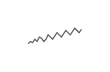
\begin{tikzpicture}[x=0.08em, y=0.08em, line width=0.4pt]
                \draw[FooterGray] (0,3) -- (1,4) -- (2,3.5) -- (3,5) -- (4,4) -- (5,6) -- (6,5.5) -- (7,4) -- (8,5) -- (9,7) -- (10,6) -- (11,5) -- (12,6.5) -- (13,8) -- (14,7) -- (15,6) -- (16,7.5) -- (17,9) -- (18,8) -- (19,7) -- (20,8.5) -- (21,10) -- (22,9) -- (23,8) -- (24,9.5);
            \end{tikzpicture}%
        }%
        \hskip0.5cm%
    }%
    \vskip6pt%
}

%=============================================================================
% PACKAGES
%=============================================================================
\usepackage[utf8]{inputenc}
\DeclareUnicodeCharacter{03B1}{\ensuremath{\alpha}}
\usepackage[T1]{fontenc}
\usepackage{amsmath, amssymb, amsthm}
\usepackage{mathtools}
\usepackage{bm}
\usepackage{tikz}
\usetikzlibrary{arrows.meta, positioning, shapes, calc, decorations.pathreplacing, shadings}
\usepackage{booktabs}
\usepackage{multirow}
\usepackage{array}
\usepackage{graphicx}
\usepackage{animate}
\usepackage{hyperref}
\usepackage{colortbl}
\usepackage{listings}
\lstset{language=Python, basicstyle=\ttfamily\scriptsize, keywordstyle=\color{MainBlue}\bfseries,
  commentstyle=\color{Forest}, stringstyle=\color{Crimson}, breaklines=true,
  frame=none, backgroundcolor=\color{VeryLightGray}, xleftmargin=2mm}
\hypersetup{colorlinks=true, linkcolor=MainBlue, urlcolor=MainBlue}
\graphicspath{{../../logos/}{../../charts/}{../../photos/}}
\usepackage{xcolor}
\hfuzz=2pt  % Suppress tiny overfull warnings (<2pt)
\vfuzz=2pt  % Suppress tiny vertical overfull warnings (<2pt)
% \mathrm in the sans-serif family of the slides (beamer resets \mathrm to the serif family at \begin{document};
% this hook runs after beamer's, so WN, Var, RMSE, ... in formulas match the surrounding text)
% Bold vectors and matrices in the same sans-serif family: \mathbf{A} in sans bold (beamer's own \mathbf came out in
% medium weight), and the bold upright Greek capitals of \boldsymbol / \bm (\bSigma, \bPhi, \boldsymbol{\Theta}) in
% cmss bold: bm.sty fixes its "boldoperators" font when it is loaded (serif cmbx), before beamer switches the
% operators to cmss, so it is reset here.
\AtBeginDocument{%
  \SetMathAlphabet{\mathrm}{normal}{\encodingdefault}{\sfdefault}{\mddefault}{n}%
  \SetMathAlphabet{\mathrm}{bold}{\encodingdefault}{\sfdefault}{bx}{n}%
  \SetMathAlphabet{\mathbf}{normal}{\encodingdefault}{\sfdefault}{bx}{n}%
  \SetMathAlphabet{\mathbf}{bold}{\encodingdefault}{\sfdefault}{bx}{n}%
  \SetSymbolFont{boldoperators}{normal}{OT1}{cmss}{bx}{n}%
  \SetSymbolFont{boldoperators}{bold}{OT1}{cmss}{bx}{n}}

%=============================================================================
% QUANTLET COMMANDS
%   \quantlet{<displayed name>}{<url>}       (generic, compatible with the older TSA decks)
%   \tsaquantlet{Ch_05}{TSA_ch5_garch}       -> https://github.com/danpele/Time-Series-Analysis/tree/main/Quantlets/Ch_05/TSA_ch5_garch
%   \qlurl{<folder>} is defined per chapter by the generator (Quantlets/Ch_NN/<folder>)
%=============================================================================
\newcommand{\tsarepo}{https://github.com/danpele/Time-Series-Analysis}
\newcommand{\tsaqlbase}{https://github.com/danpele/Time-Series-Analysis/tree/main/Quantlets}
\newcommand{\quantlet}[2]{%
    \hfill\href{#2}{%
        \raisebox{-0.15em}{
\includegraphics[height=0.7em]{ql_logo.png}}%
        \textcolor{MainBlue}{\tiny\ #1}%
    }%
}
\newcommand{\tsaquantlet}[2]{\quantlet{\detokenize{#2}}{\tsaqlbase/#1/#2}}

%=============================================================================
% NOTEBOOKS (Google Colab)
%   \colaburl{notebooks/EN/chapter5_seminar_notebook.ipynb} -> the Colab link of a file in the TSA repo
%   \nb: the chapter notebook (each seminar deck redefines it with \renewcommand)
%=============================================================================
\newcommand{\colaburl}[1]{https://colab.research.google.com/github/danpele/Time-Series-Analysis/blob/main/#1}
\newcommand{\nb}{https://colab.research.google.com/github/danpele/Time-Series-Analysis/tree/main/notebooks/EN}
\newcommand{\nbname}{notebooks/EN}

%=============================================================================
% SLIDE HELPERS (used by the generators; the same as in MFM)
%=============================================================================
% local font size for list bodies (the preamble forces \normalsize)
\newcommand{\itemsize}[1]{\setbeamertemplate{itemize/enumerate body begin}{#1}\setbeamertemplate{itemize/enumerate subbody begin}{#1}}
\newcommand{\intitle}[1]{{\hypersetup{urlcolor=white}#1}}   % white links inside coloured title bars
\newcommand{\imgcap}[1]{{\scriptsize #1}\\[0.5mm]}          % caption under a photo
\newcommand{\imgcredit}[2]{{\tiny\color{FooterGray}\href{#1}{#2}}}   % image credit: source URL, author/licence
\newcommand{\aiprompt}[1]{{\ttfamily\color{MainBlue}#1}}     % a prompt to an AI assistant

%=============================================================================
% SEMINARS: student version by default; the instructor wrapper *_solutions.tex sets \solutionstrue
%=============================================================================
\makeatletter\@ifundefined{ifsolutions}{\expandafter\newif\csname ifsolutions\endcsname}{}\makeatother
\newcommand{\solonly}[1]{\ifsolutions #1\fi}
\newcommand{\propsub}{\ifsolutions\else\framesubtitle{\ifdefined\tsalang Rezolvarea se discută la seminar\else Solution discussed in class\fi}\fi}

%=============================================================================
% APPENDIX AND CHAPTER LINKS (latex/appendix_links.py writes the calls; it also re-declares these
% macros before \begin{document}, so the decks compile with or without this preamble block)
%=============================================================================
\providecommand{\tsaapplink}[3]{\hypertarget{#2}{}\hyperlink{#1}{\beamergotobutton{#3}}}
\providecommand{\tsaappback}[2]{\begin{tikzpicture}[remember picture,overlay]\node[anchor=south east] at ([xshift=-3mm,yshift=7mm]current page.south east){\hyperlink{#1}{\beamerreturnbutton{#2}}};\end{tikzpicture}}
\providecommand{\tsachlink}[2]{\href{#1}{#2}}
\providecommand{\tsachlinkt}[2]{\href{#1}{\usebeamercolor[fg]{frametitle}#2}}

%=============================================================================
% QUANTINAR COMMAND: link către un curs Quantinar (subiecte avansate)
%=============================================================================
\newcommand{\quantinar}[2]{%
    \href{#2}{%
        \raisebox{-0.15em}{
\includegraphics[height=0.8em]{qr_logo.png}}%
        \textcolor{MainBlue}{\scriptsize\ #1}%
    }%
}

%=============================================================================
% CUSTOM TITLE PAGE
%=============================================================================
\defbeamertemplate*{title page}{hybrid}[1][]
{
    \vspace{0.2cm}
    % Logos row - top header (with clickable links)
    \begin{center}
        \href{https://www.ase.ro}{
\includegraphics[height=1.0cm]{ase_logo.png}}\hspace{0.3cm}%
        \href{https://theida.net}{
\includegraphics[height=1.0cm]{ida_logo.png}}\hspace{0.3cm}%
        \href{https://blockchain-research-center.com}{
\includegraphics[height=1.0cm]{brc_logo.png}}\hspace{0.3cm}%
        \href{https://www.ai4efin.ase.ro}{
\includegraphics[height=1.0cm]{ai4efin_logo.png}}\hspace{0.3cm}%
        \href{https://ipe.ro/new}{
\includegraphics[height=1.0cm]{acad_logo.png}}\hspace{0.3cm}%
        \href{https://www.digital-finance-msca.com}{
\includegraphics[height=1.0cm]{msca_logo.png}}%
    \end{center}

    \vspace{0.6cm}

    % Main title with Q logos on sides (with clickable links)
    \begin{center}
        \begin{minipage}{0.1\textwidth}
            \centering
            \href{https://quantlet.com}{
\includegraphics[height=1.1cm]{ql_logo.png}}
        \end{minipage}%
        \begin{minipage}{0.78\textwidth}
            \centering
            {\LARGE\bfseries\usebeamercolor[fg]{title}\inserttitle}

            \vspace{0.3cm}

            {\usebeamerfont{subtitle}\usebeamercolor[fg]{title}\insertsubtitle}
        \end{minipage}%
        \begin{minipage}{0.1\textwidth}
            \centering
            \href{https://quantinar.com}{
\includegraphics[height=1.1cm]{qr_logo.png}}
        \end{minipage}
    \end{center}

    \vspace{0.6cm}

    % Authors (left aligned)
    \hspace{0.5cm}{\usebeamerfont{author}\insertauthor}

    \vspace{0.3cm}

    % Institute/Affiliations (left aligned)
    \hspace{0.5cm}\begin{minipage}[t]{0.9\textwidth}
        \raggedright\small\insertinstitute
    \end{minipage}
}

%=============================================================================
% THEOREM ENVIRONMENTS
%=============================================================================
\theoremstyle{definition}
\setbeamertemplate{theorems}[numbered]
\ifdefined\tsalang
\newtheorem{defn}{Definiție}
\newtheorem{thm}{Teoremă}
\newtheorem{prop}{Propoziție}
\newtheorem{rmk}{Observație}
\else
\newtheorem{defn}{Definition}
\newtheorem{thm}{Theorem}
\newtheorem{prop}{Proposition}
\newtheorem{rmk}{Remark}
\fi

%=============================================================================
% CENTRED MINIPAGE (no extra vertical space)
%=============================================================================
\newenvironment{cminipage}[1]{%
    \par\noindent\hfill\begin{minipage}{#1}\ignorespaces
}{%
    \end{minipage}\hfill\null\par
}

%=============================================================================
% CUSTOM COMMANDS
%=============================================================================
\newcommand{\E}{\mathbb{E}}
\newcommand{\Var}{\text{Var}}
\newcommand{\Cov}{\text{Cov}}
\newcommand{\Corr}{\text{Corr}}
\newcommand{\R}{\mathbb{R}}
\newcommand{\N}{\mathbb{N}}
\newcommand{\Z}{\mathbb{Z}}
\newcommand{\B}{\mathbf{B}}
\newcommand{\imark}{\textcolor{MainBlue}{\textbullet}}
\newcommand{\RMSE}{\text{RMSE}}
\newcommand{\MAE}{\text{MAE}}
\newcommand{\MAPE}{\text{MAPE}}

% Boldface vector/matrix commands (VAR, VECM, state space; also used by the older TSA decks)
\newcommand{\bY}{\mathbf{Y}}
\newcommand{\bX}{\mathbf{X}}
\newcommand{\bA}{\mathbf{A}}
\newcommand{\bB}{\mathbf{B}}
\newcommand{\bepsilon}{\boldsymbol{\varepsilon}}
\newcommand{\bSigma}{\boldsymbol{\Sigma}}
\newcommand{\bPhi}{\boldsymbol{\Phi}}
\newcommand{\bGamma}{\boldsymbol{\Gamma}}
\newcommand{\bPi}{\boldsymbol{\Pi}}
\newcommand{\bc}{\mathbf{c}}
\newcommand{\balpha}{\boldsymbol{\alpha}}
\newcommand{\bbeta}{\boldsymbol{\beta}}
\newcommand{\bvarepsilon}{\boldsymbol{\varepsilon}}

% Legacy seminar marks (older TSA seminar decks)
\newcommand{\correct}{\textcolor{Forest}{\checkmark}}
\newcommand{\incorrect}{\textcolor{Crimson}{\texttimes}}
 se definește
%   \newcommand{\coursename}{Time Series Analysis}      (EN)
%   \newcommand{\coursename}{Serii de timp}       (RO)  și  \def\tsalang{ro}
% Fișierele .tex se află în EN/Courses, EN/Seminars, RO/Cursuri, RO/Seminarii (două niveluri sub rădăcină).
% Deck-urile sînt generate de latex/build_chapterN.py / build_seminarN.py (vezi latex/tsa_build.py).

\documentclass[9pt, aspectratio=169, t]{beamer}
\providecommand{\coursename}{Time Series Analysis}

% Ensure content fits on slides
\setbeamersize{text margin left=8mm, text margin right=8mm}
% Smaller institute font (title page)
\setbeamerfont{institute}{size=\footnotesize}

%=============================================================================
% THEME AND STYLE CONFIGURATION
%=============================================================================
\usetheme{default}
% Using default theme for clean header/footer control

% Color Palette (matching Redispatch PDF)
\definecolor{MainBlue}{RGB}{26, 58, 110}
\definecolor{AccentBlue}{RGB}{26, 58, 110}
\definecolor{IDAred}{RGB}{205, 0, 0}
\definecolor{DarkGray}{RGB}{51, 51, 51}
\definecolor{MediumGray}{RGB}{128, 128, 128}
\definecolor{LightGray}{RGB}{248, 248, 248}
\definecolor{VeryLightGray}{RGB}{235, 235, 235}
\definecolor{KeynoteGray}{RGB}{218, 218, 218}
\definecolor{SectionGray}{RGB}{120, 120, 120}
\definecolor{FooterGray}{RGB}{100, 100, 100}
\definecolor{Crimson}{RGB}{220, 53, 69}
\definecolor{Forest}{RGB}{46, 125, 50}
\definecolor{Amber}{RGB}{181, 133, 63}
\definecolor{Orange}{RGB}{230, 126, 34}
\definecolor{Purple}{RGB}{142, 68, 173}

% Gradient background (exact Keynote 315° gradient: white to RGB 218,218,218)
\setbeamertemplate{background}{%
    \begin{tikzpicture}[remember picture, overlay]
        \shade[shading=axis, shading angle=315,
        top color=white, bottom color=KeynoteGray]
        (current page.south west) rectangle (current page.north east);
    \end{tikzpicture}%
}
% Fallback solid color for compatibility
\setbeamercolor{background canvas}{bg=}

\setbeamercolor{palette primary}{bg=MainBlue, fg=white}
\setbeamercolor{palette secondary}{bg=MainBlue!85, fg=white}
\setbeamercolor{palette tertiary}{bg=MainBlue!70, fg=white}
\setbeamercolor{structure}{fg=MainBlue}
\setbeamercolor{title}{fg=IDAred}
\setbeamercolor{frametitle}{fg=IDAred, bg=}
\setbeamercolor{block title}{bg=MainBlue, fg=white}
\setbeamercolor{block body}{bg=VeryLightGray, fg=DarkGray}
\setbeamercolor{block title alerted}{bg=Crimson, fg=white}
\setbeamercolor{block body alerted}{bg=Crimson!8, fg=DarkGray}
\setbeamercolor{block title example}{bg=Forest, fg=white}
\setbeamercolor{block body example}{bg=Forest!8, fg=DarkGray}
\setbeamercolor{item}{fg=MainBlue}

% Footer colors (override Madrid theme blue)
\setbeamercolor{author in head/foot}{fg=FooterGray, bg=}
\setbeamercolor{title in head/foot}{fg=FooterGray, bg=}
\setbeamercolor{date in head/foot}{fg=FooterGray, bg=}
\setbeamercolor{section in head/foot}{fg=FooterGray, bg=}
\setbeamercolor{subsection in head/foot}{fg=FooterGray, bg=}

% Bullet styles (apply everywhere including blocks)
\setbeamertemplate{itemize item}{\color{MainBlue}$\boxdot$}
\setbeamertemplate{itemize subitem}{\color{MainBlue}$\blacktriangleright$}
\setbeamertemplate{itemize subsubitem}{\color{MainBlue}\tiny$\bullet$}
\setbeamertemplate{itemize/enumerate body begin}{\normalsize}
\setbeamertemplate{itemize/enumerate subbody begin}{\normalsize}

% Item spacing - compact style
\setlength{\leftmargini}{10pt}       % Level 1: minimal indent
\setlength{\leftmarginii}{10pt}      % Level 2: minimal additional indent
% Compact list spacing (zero extra space before/after lists in blocks)
\makeatletter
\def\@listi{\leftmargin\leftmargini \topsep 0pt \parsep 0pt \itemsep 0pt}
\def\@listii{\leftmargin\leftmarginii \topsep 0pt \parsep 0pt \itemsep 0pt}
\makeatother

\setbeamertemplate{navigation symbols}{}

%=============================================================================
% CUSTOM HEADLINE
%=============================================================================
\setbeamertemplate{headline}{%
    \vskip10pt%
    \hbox to \paperwidth{%
        \hskip0.5cm%
        {\small\color{FooterGray}\renewcommand{\hyperlink}[2]{##2}\insertsectionhead}%
        \hfill%
        \textcolor{FooterGray}{\small\insertframenumber}%
        \hskip0.5cm%
    }%
    \vskip4pt%
    {\color{FooterGray}\hrule height 0.4pt}%
}

%=============================================================================
% CUSTOM FOOTER
%=============================================================================
\usepackage{fontawesome5}

\setbeamertemplate{footline}{%
    {\color{FooterGray}\hrule height 0.4pt}%
    \vskip4pt%
    \hbox to \paperwidth{%
        \hskip0.5cm%
        \textcolor{FooterGray}{\small\coursename}%
        \hfill%
        \raisebox{-0.1em}{%
            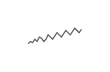
\begin{tikzpicture}[x=0.08em, y=0.08em, line width=0.4pt]
                \draw[FooterGray] (0,3) -- (1,4) -- (2,3.5) -- (3,5) -- (4,4) -- (5,6) -- (6,5.5) -- (7,4) -- (8,5) -- (9,7) -- (10,6) -- (11,5) -- (12,6.5) -- (13,8) -- (14,7) -- (15,6) -- (16,7.5) -- (17,9) -- (18,8) -- (19,7) -- (20,8.5) -- (21,10) -- (22,9) -- (23,8) -- (24,9.5);
            \end{tikzpicture}%
        }%
        \hskip0.5cm%
    }%
    \vskip6pt%
}

%=============================================================================
% PACKAGES
%=============================================================================
\usepackage[utf8]{inputenc}
\DeclareUnicodeCharacter{03B1}{\ensuremath{\alpha}}
\usepackage[T1]{fontenc}
\usepackage{amsmath, amssymb, amsthm}
\usepackage{mathtools}
\usepackage{bm}
\usepackage{tikz}
\usetikzlibrary{arrows.meta, positioning, shapes, calc, decorations.pathreplacing, shadings}
\usepackage{booktabs}
\usepackage{multirow}
\usepackage{array}
\usepackage{graphicx}
\usepackage{animate}
\usepackage{hyperref}
\usepackage{colortbl}
\usepackage{listings}
\lstset{language=Python, basicstyle=\ttfamily\scriptsize, keywordstyle=\color{MainBlue}\bfseries,
  commentstyle=\color{Forest}, stringstyle=\color{Crimson}, breaklines=true,
  frame=none, backgroundcolor=\color{VeryLightGray}, xleftmargin=2mm}
\hypersetup{colorlinks=true, linkcolor=MainBlue, urlcolor=MainBlue}
\graphicspath{{../../logos/}{../../charts/}{../../photos/}}
\usepackage{xcolor}
\hfuzz=2pt  % Suppress tiny overfull warnings (<2pt)
\vfuzz=2pt  % Suppress tiny vertical overfull warnings (<2pt)
% \mathrm in the sans-serif family of the slides (beamer resets \mathrm to the serif family at \begin{document};
% this hook runs after beamer's, so WN, Var, RMSE, ... in formulas match the surrounding text)
% Bold vectors and matrices in the same sans-serif family: \mathbf{A} in sans bold (beamer's own \mathbf came out in
% medium weight), and the bold upright Greek capitals of \boldsymbol / \bm (\bSigma, \bPhi, \boldsymbol{\Theta}) in
% cmss bold: bm.sty fixes its "boldoperators" font when it is loaded (serif cmbx), before beamer switches the
% operators to cmss, so it is reset here.
\AtBeginDocument{%
  \SetMathAlphabet{\mathrm}{normal}{\encodingdefault}{\sfdefault}{\mddefault}{n}%
  \SetMathAlphabet{\mathrm}{bold}{\encodingdefault}{\sfdefault}{bx}{n}%
  \SetMathAlphabet{\mathbf}{normal}{\encodingdefault}{\sfdefault}{bx}{n}%
  \SetMathAlphabet{\mathbf}{bold}{\encodingdefault}{\sfdefault}{bx}{n}%
  \SetSymbolFont{boldoperators}{normal}{OT1}{cmss}{bx}{n}%
  \SetSymbolFont{boldoperators}{bold}{OT1}{cmss}{bx}{n}}

%=============================================================================
% QUANTLET COMMANDS
%   \quantlet{<displayed name>}{<url>}       (generic, compatible with the older TSA decks)
%   \tsaquantlet{Ch_05}{TSA_ch5_garch}       -> https://github.com/danpele/Time-Series-Analysis/tree/main/Quantlets/Ch_05/TSA_ch5_garch
%   \qlurl{<folder>} is defined per chapter by the generator (Quantlets/Ch_NN/<folder>)
%=============================================================================
\newcommand{\tsarepo}{https://github.com/danpele/Time-Series-Analysis}
\newcommand{\tsaqlbase}{https://github.com/danpele/Time-Series-Analysis/tree/main/Quantlets}
\newcommand{\quantlet}[2]{%
    \hfill\href{#2}{%
        \raisebox{-0.15em}{
\includegraphics[height=0.7em]{ql_logo.png}}%
        \textcolor{MainBlue}{\tiny\ #1}%
    }%
}
\newcommand{\tsaquantlet}[2]{\quantlet{\detokenize{#2}}{\tsaqlbase/#1/#2}}

%=============================================================================
% NOTEBOOKS (Google Colab)
%   \colaburl{notebooks/EN/chapter5_seminar_notebook.ipynb} -> the Colab link of a file in the TSA repo
%   \nb: the chapter notebook (each seminar deck redefines it with \renewcommand)
%=============================================================================
\newcommand{\colaburl}[1]{https://colab.research.google.com/github/danpele/Time-Series-Analysis/blob/main/#1}
\newcommand{\nb}{https://colab.research.google.com/github/danpele/Time-Series-Analysis/tree/main/notebooks/EN}
\newcommand{\nbname}{notebooks/EN}

%=============================================================================
% SLIDE HELPERS (used by the generators; the same as in MFM)
%=============================================================================
% local font size for list bodies (the preamble forces \normalsize)
\newcommand{\itemsize}[1]{\setbeamertemplate{itemize/enumerate body begin}{#1}\setbeamertemplate{itemize/enumerate subbody begin}{#1}}
\newcommand{\intitle}[1]{{\hypersetup{urlcolor=white}#1}}   % white links inside coloured title bars
\newcommand{\imgcap}[1]{{\scriptsize #1}\\[0.5mm]}          % caption under a photo
\newcommand{\imgcredit}[2]{{\tiny\color{FooterGray}\href{#1}{#2}}}   % image credit: source URL, author/licence
\newcommand{\aiprompt}[1]{{\ttfamily\color{MainBlue}#1}}     % a prompt to an AI assistant

%=============================================================================
% SEMINARS: student version by default; the instructor wrapper *_solutions.tex sets \solutionstrue
%=============================================================================
\makeatletter\@ifundefined{ifsolutions}{\expandafter\newif\csname ifsolutions\endcsname}{}\makeatother
\newcommand{\solonly}[1]{\ifsolutions #1\fi}
\newcommand{\propsub}{\ifsolutions\else\framesubtitle{\ifdefined\tsalang Rezolvarea se discută la seminar\else Solution discussed in class\fi}\fi}

%=============================================================================
% APPENDIX AND CHAPTER LINKS (latex/appendix_links.py writes the calls; it also re-declares these
% macros before \begin{document}, so the decks compile with or without this preamble block)
%=============================================================================
\providecommand{\tsaapplink}[3]{\hypertarget{#2}{}\hyperlink{#1}{\beamergotobutton{#3}}}
\providecommand{\tsaappback}[2]{\begin{tikzpicture}[remember picture,overlay]\node[anchor=south east] at ([xshift=-3mm,yshift=7mm]current page.south east){\hyperlink{#1}{\beamerreturnbutton{#2}}};\end{tikzpicture}}
\providecommand{\tsachlink}[2]{\href{#1}{#2}}
\providecommand{\tsachlinkt}[2]{\href{#1}{\usebeamercolor[fg]{frametitle}#2}}

%=============================================================================
% QUANTINAR COMMAND: link către un curs Quantinar (subiecte avansate)
%=============================================================================
\newcommand{\quantinar}[2]{%
    \href{#2}{%
        \raisebox{-0.15em}{
\includegraphics[height=0.8em]{qr_logo.png}}%
        \textcolor{MainBlue}{\scriptsize\ #1}%
    }%
}

%=============================================================================
% CUSTOM TITLE PAGE
%=============================================================================
\defbeamertemplate*{title page}{hybrid}[1][]
{
    \vspace{0.2cm}
    % Logos row - top header (with clickable links)
    \begin{center}
        \href{https://www.ase.ro}{
\includegraphics[height=1.0cm]{ase_logo.png}}\hspace{0.3cm}%
        \href{https://theida.net}{
\includegraphics[height=1.0cm]{ida_logo.png}}\hspace{0.3cm}%
        \href{https://blockchain-research-center.com}{
\includegraphics[height=1.0cm]{brc_logo.png}}\hspace{0.3cm}%
        \href{https://www.ai4efin.ase.ro}{
\includegraphics[height=1.0cm]{ai4efin_logo.png}}\hspace{0.3cm}%
        \href{https://ipe.ro/new}{
\includegraphics[height=1.0cm]{acad_logo.png}}\hspace{0.3cm}%
        \href{https://www.digital-finance-msca.com}{
\includegraphics[height=1.0cm]{msca_logo.png}}%
    \end{center}

    \vspace{0.6cm}

    % Main title with Q logos on sides (with clickable links)
    \begin{center}
        \begin{minipage}{0.1\textwidth}
            \centering
            \href{https://quantlet.com}{
\includegraphics[height=1.1cm]{ql_logo.png}}
        \end{minipage}%
        \begin{minipage}{0.78\textwidth}
            \centering
            {\LARGE\bfseries\usebeamercolor[fg]{title}\inserttitle}

            \vspace{0.3cm}

            {\usebeamerfont{subtitle}\usebeamercolor[fg]{title}\insertsubtitle}
        \end{minipage}%
        \begin{minipage}{0.1\textwidth}
            \centering
            \href{https://quantinar.com}{
\includegraphics[height=1.1cm]{qr_logo.png}}
        \end{minipage}
    \end{center}

    \vspace{0.6cm}

    % Authors (left aligned)
    \hspace{0.5cm}{\usebeamerfont{author}\insertauthor}

    \vspace{0.3cm}

    % Institute/Affiliations (left aligned)
    \hspace{0.5cm}\begin{minipage}[t]{0.9\textwidth}
        \raggedright\small\insertinstitute
    \end{minipage}
}

%=============================================================================
% THEOREM ENVIRONMENTS
%=============================================================================
\theoremstyle{definition}
\setbeamertemplate{theorems}[numbered]
\ifdefined\tsalang
\newtheorem{defn}{Definiție}
\newtheorem{thm}{Teoremă}
\newtheorem{prop}{Propoziție}
\newtheorem{rmk}{Observație}
\else
\newtheorem{defn}{Definition}
\newtheorem{thm}{Theorem}
\newtheorem{prop}{Proposition}
\newtheorem{rmk}{Remark}
\fi

%=============================================================================
% CENTRED MINIPAGE (no extra vertical space)
%=============================================================================
\newenvironment{cminipage}[1]{%
    \par\noindent\hfill\begin{minipage}{#1}\ignorespaces
}{%
    \end{minipage}\hfill\null\par
}

%=============================================================================
% CUSTOM COMMANDS
%=============================================================================
\newcommand{\E}{\mathbb{E}}
\newcommand{\Var}{\text{Var}}
\newcommand{\Cov}{\text{Cov}}
\newcommand{\Corr}{\text{Corr}}
\newcommand{\R}{\mathbb{R}}
\newcommand{\N}{\mathbb{N}}
\newcommand{\Z}{\mathbb{Z}}
\newcommand{\B}{\mathbf{B}}
\newcommand{\imark}{\textcolor{MainBlue}{\textbullet}}
\newcommand{\RMSE}{\text{RMSE}}
\newcommand{\MAE}{\text{MAE}}
\newcommand{\MAPE}{\text{MAPE}}

% Boldface vector/matrix commands (VAR, VECM, state space; also used by the older TSA decks)
\newcommand{\bY}{\mathbf{Y}}
\newcommand{\bX}{\mathbf{X}}
\newcommand{\bA}{\mathbf{A}}
\newcommand{\bB}{\mathbf{B}}
\newcommand{\bepsilon}{\boldsymbol{\varepsilon}}
\newcommand{\bSigma}{\boldsymbol{\Sigma}}
\newcommand{\bPhi}{\boldsymbol{\Phi}}
\newcommand{\bGamma}{\boldsymbol{\Gamma}}
\newcommand{\bPi}{\boldsymbol{\Pi}}
\newcommand{\bc}{\mathbf{c}}
\newcommand{\balpha}{\boldsymbol{\alpha}}
\newcommand{\bbeta}{\boldsymbol{\beta}}
\newcommand{\bvarepsilon}{\boldsymbol{\varepsilon}}

% Legacy seminar marks (older TSA seminar decks)
\newcommand{\correct}{\textcolor{Forest}{\checkmark}}
\newcommand{\incorrect}{\textcolor{Crimson}{\texttimes}}
 se definește
%   \newcommand{\coursename}{Time Series Analysis}      (EN)
%   \newcommand{\coursename}{Serii de timp}       (RO)  și  \def\tsalang{ro}
% Fișierele .tex se află în EN/Courses, EN/Seminars, RO/Cursuri, RO/Seminarii (două niveluri sub rădăcină).
% Deck-urile sînt generate de latex/build_chapterN.py / build_seminarN.py (vezi latex/tsa_build.py).

\documentclass[9pt, aspectratio=169, t]{beamer}
\providecommand{\coursename}{Time Series Analysis}

% Ensure content fits on slides
\setbeamersize{text margin left=8mm, text margin right=8mm}
% Smaller institute font (title page)
\setbeamerfont{institute}{size=\footnotesize}

%=============================================================================
% THEME AND STYLE CONFIGURATION
%=============================================================================
\usetheme{default}
% Using default theme for clean header/footer control

% Color Palette (matching Redispatch PDF)
\definecolor{MainBlue}{RGB}{26, 58, 110}
\definecolor{AccentBlue}{RGB}{26, 58, 110}
\definecolor{IDAred}{RGB}{205, 0, 0}
\definecolor{DarkGray}{RGB}{51, 51, 51}
\definecolor{MediumGray}{RGB}{128, 128, 128}
\definecolor{LightGray}{RGB}{248, 248, 248}
\definecolor{VeryLightGray}{RGB}{235, 235, 235}
\definecolor{KeynoteGray}{RGB}{218, 218, 218}
\definecolor{SectionGray}{RGB}{120, 120, 120}
\definecolor{FooterGray}{RGB}{100, 100, 100}
\definecolor{Crimson}{RGB}{220, 53, 69}
\definecolor{Forest}{RGB}{46, 125, 50}
\definecolor{Amber}{RGB}{181, 133, 63}
\definecolor{Orange}{RGB}{230, 126, 34}
\definecolor{Purple}{RGB}{142, 68, 173}

% Gradient background (exact Keynote 315° gradient: white to RGB 218,218,218)
\setbeamertemplate{background}{%
    \begin{tikzpicture}[remember picture, overlay]
        \shade[shading=axis, shading angle=315,
        top color=white, bottom color=KeynoteGray]
        (current page.south west) rectangle (current page.north east);
    \end{tikzpicture}%
}
% Fallback solid color for compatibility
\setbeamercolor{background canvas}{bg=}

\setbeamercolor{palette primary}{bg=MainBlue, fg=white}
\setbeamercolor{palette secondary}{bg=MainBlue!85, fg=white}
\setbeamercolor{palette tertiary}{bg=MainBlue!70, fg=white}
\setbeamercolor{structure}{fg=MainBlue}
\setbeamercolor{title}{fg=IDAred}
\setbeamercolor{frametitle}{fg=IDAred, bg=}
\setbeamercolor{block title}{bg=MainBlue, fg=white}
\setbeamercolor{block body}{bg=VeryLightGray, fg=DarkGray}
\setbeamercolor{block title alerted}{bg=Crimson, fg=white}
\setbeamercolor{block body alerted}{bg=Crimson!8, fg=DarkGray}
\setbeamercolor{block title example}{bg=Forest, fg=white}
\setbeamercolor{block body example}{bg=Forest!8, fg=DarkGray}
\setbeamercolor{item}{fg=MainBlue}

% Footer colors (override Madrid theme blue)
\setbeamercolor{author in head/foot}{fg=FooterGray, bg=}
\setbeamercolor{title in head/foot}{fg=FooterGray, bg=}
\setbeamercolor{date in head/foot}{fg=FooterGray, bg=}
\setbeamercolor{section in head/foot}{fg=FooterGray, bg=}
\setbeamercolor{subsection in head/foot}{fg=FooterGray, bg=}

% Bullet styles (apply everywhere including blocks)
\setbeamertemplate{itemize item}{\color{MainBlue}$\boxdot$}
\setbeamertemplate{itemize subitem}{\color{MainBlue}$\blacktriangleright$}
\setbeamertemplate{itemize subsubitem}{\color{MainBlue}\tiny$\bullet$}
\setbeamertemplate{itemize/enumerate body begin}{\normalsize}
\setbeamertemplate{itemize/enumerate subbody begin}{\normalsize}

% Item spacing - compact style
\setlength{\leftmargini}{10pt}       % Level 1: minimal indent
\setlength{\leftmarginii}{10pt}      % Level 2: minimal additional indent
% Compact list spacing (zero extra space before/after lists in blocks)
\makeatletter
\def\@listi{\leftmargin\leftmargini \topsep 0pt \parsep 0pt \itemsep 0pt}
\def\@listii{\leftmargin\leftmarginii \topsep 0pt \parsep 0pt \itemsep 0pt}
\makeatother

\setbeamertemplate{navigation symbols}{}

%=============================================================================
% CUSTOM HEADLINE
%=============================================================================
\setbeamertemplate{headline}{%
    \vskip10pt%
    \hbox to \paperwidth{%
        \hskip0.5cm%
        {\small\color{FooterGray}\renewcommand{\hyperlink}[2]{##2}\insertsectionhead}%
        \hfill%
        \textcolor{FooterGray}{\small\insertframenumber}%
        \hskip0.5cm%
    }%
    \vskip4pt%
    {\color{FooterGray}\hrule height 0.4pt}%
}

%=============================================================================
% CUSTOM FOOTER
%=============================================================================
\usepackage{fontawesome5}

\setbeamertemplate{footline}{%
    {\color{FooterGray}\hrule height 0.4pt}%
    \vskip4pt%
    \hbox to \paperwidth{%
        \hskip0.5cm%
        \textcolor{FooterGray}{\small\coursename}%
        \hfill%
        \raisebox{-0.1em}{%
            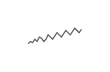
\begin{tikzpicture}[x=0.08em, y=0.08em, line width=0.4pt]
                \draw[FooterGray] (0,3) -- (1,4) -- (2,3.5) -- (3,5) -- (4,4) -- (5,6) -- (6,5.5) -- (7,4) -- (8,5) -- (9,7) -- (10,6) -- (11,5) -- (12,6.5) -- (13,8) -- (14,7) -- (15,6) -- (16,7.5) -- (17,9) -- (18,8) -- (19,7) -- (20,8.5) -- (21,10) -- (22,9) -- (23,8) -- (24,9.5);
            \end{tikzpicture}%
        }%
        \hskip0.5cm%
    }%
    \vskip6pt%
}

%=============================================================================
% PACKAGES
%=============================================================================
\usepackage[utf8]{inputenc}
\DeclareUnicodeCharacter{03B1}{\ensuremath{\alpha}}
\usepackage[T1]{fontenc}
\usepackage{amsmath, amssymb, amsthm}
\usepackage{mathtools}
\usepackage{bm}
\usepackage{tikz}
\usetikzlibrary{arrows.meta, positioning, shapes, calc, decorations.pathreplacing, shadings}
\usepackage{booktabs}
\usepackage{multirow}
\usepackage{array}
\usepackage{graphicx}
\usepackage{animate}
\usepackage{hyperref}
\usepackage{colortbl}
\usepackage{listings}
\lstset{language=Python, basicstyle=\ttfamily\scriptsize, keywordstyle=\color{MainBlue}\bfseries,
  commentstyle=\color{Forest}, stringstyle=\color{Crimson}, breaklines=true,
  frame=none, backgroundcolor=\color{VeryLightGray}, xleftmargin=2mm}
\hypersetup{colorlinks=true, linkcolor=MainBlue, urlcolor=MainBlue}
\graphicspath{{../../logos/}{../../charts/}{../../photos/}}
\usepackage{xcolor}
\hfuzz=2pt  % Suppress tiny overfull warnings (<2pt)
\vfuzz=2pt  % Suppress tiny vertical overfull warnings (<2pt)
% \mathrm in the sans-serif family of the slides (beamer resets \mathrm to the serif family at \begin{document};
% this hook runs after beamer's, so WN, Var, RMSE, ... in formulas match the surrounding text)
% Bold vectors and matrices in the same sans-serif family: \mathbf{A} in sans bold (beamer's own \mathbf came out in
% medium weight), and the bold upright Greek capitals of \boldsymbol / \bm (\bSigma, \bPhi, \boldsymbol{\Theta}) in
% cmss bold: bm.sty fixes its "boldoperators" font when it is loaded (serif cmbx), before beamer switches the
% operators to cmss, so it is reset here.
\AtBeginDocument{%
  \SetMathAlphabet{\mathrm}{normal}{\encodingdefault}{\sfdefault}{\mddefault}{n}%
  \SetMathAlphabet{\mathrm}{bold}{\encodingdefault}{\sfdefault}{bx}{n}%
  \SetMathAlphabet{\mathbf}{normal}{\encodingdefault}{\sfdefault}{bx}{n}%
  \SetMathAlphabet{\mathbf}{bold}{\encodingdefault}{\sfdefault}{bx}{n}%
  \SetSymbolFont{boldoperators}{normal}{OT1}{cmss}{bx}{n}%
  \SetSymbolFont{boldoperators}{bold}{OT1}{cmss}{bx}{n}}

%=============================================================================
% QUANTLET COMMANDS
%   \quantlet{<displayed name>}{<url>}       (generic, compatible with the older TSA decks)
%   \tsaquantlet{Ch_05}{TSA_ch5_garch}       -> https://github.com/danpele/Time-Series-Analysis/tree/main/Quantlets/Ch_05/TSA_ch5_garch
%   \qlurl{<folder>} is defined per chapter by the generator (Quantlets/Ch_NN/<folder>)
%=============================================================================
\newcommand{\tsarepo}{https://github.com/danpele/Time-Series-Analysis}
\newcommand{\tsaqlbase}{https://github.com/danpele/Time-Series-Analysis/tree/main/Quantlets}
\newcommand{\quantlet}[2]{%
    \hfill\href{#2}{%
        \raisebox{-0.15em}{
\includegraphics[height=0.7em]{ql_logo.png}}%
        \textcolor{MainBlue}{\tiny\ #1}%
    }%
}
\newcommand{\tsaquantlet}[2]{\quantlet{\detokenize{#2}}{\tsaqlbase/#1/#2}}

%=============================================================================
% NOTEBOOKS (Google Colab)
%   \colaburl{notebooks/EN/chapter5_seminar_notebook.ipynb} -> the Colab link of a file in the TSA repo
%   \nb: the chapter notebook (each seminar deck redefines it with \renewcommand)
%=============================================================================
\newcommand{\colaburl}[1]{https://colab.research.google.com/github/danpele/Time-Series-Analysis/blob/main/#1}
\newcommand{\nb}{https://colab.research.google.com/github/danpele/Time-Series-Analysis/tree/main/notebooks/EN}
\newcommand{\nbname}{notebooks/EN}

%=============================================================================
% SLIDE HELPERS (used by the generators; the same as in MFM)
%=============================================================================
% local font size for list bodies (the preamble forces \normalsize)
\newcommand{\itemsize}[1]{\setbeamertemplate{itemize/enumerate body begin}{#1}\setbeamertemplate{itemize/enumerate subbody begin}{#1}}
\newcommand{\intitle}[1]{{\hypersetup{urlcolor=white}#1}}   % white links inside coloured title bars
\newcommand{\imgcap}[1]{{\scriptsize #1}\\[0.5mm]}          % caption under a photo
\newcommand{\imgcredit}[2]{{\tiny\color{FooterGray}\href{#1}{#2}}}   % image credit: source URL, author/licence
\newcommand{\aiprompt}[1]{{\ttfamily\color{MainBlue}#1}}     % a prompt to an AI assistant

%=============================================================================
% SEMINARS: student version by default; the instructor wrapper *_solutions.tex sets \solutionstrue
%=============================================================================
\makeatletter\@ifundefined{ifsolutions}{\expandafter\newif\csname ifsolutions\endcsname}{}\makeatother
\newcommand{\solonly}[1]{\ifsolutions #1\fi}
\newcommand{\propsub}{\ifsolutions\else\framesubtitle{\ifdefined\tsalang Rezolvarea se discută la seminar\else Solution discussed in class\fi}\fi}

%=============================================================================
% APPENDIX AND CHAPTER LINKS (latex/appendix_links.py writes the calls; it also re-declares these
% macros before \begin{document}, so the decks compile with or without this preamble block)
%=============================================================================
\providecommand{\tsaapplink}[3]{\hypertarget{#2}{}\hyperlink{#1}{\beamergotobutton{#3}}}
\providecommand{\tsaappback}[2]{\begin{tikzpicture}[remember picture,overlay]\node[anchor=south east] at ([xshift=-3mm,yshift=7mm]current page.south east){\hyperlink{#1}{\beamerreturnbutton{#2}}};\end{tikzpicture}}
\providecommand{\tsachlink}[2]{\href{#1}{#2}}
\providecommand{\tsachlinkt}[2]{\href{#1}{\usebeamercolor[fg]{frametitle}#2}}

%=============================================================================
% QUANTINAR COMMAND: link către un curs Quantinar (subiecte avansate)
%=============================================================================
\newcommand{\quantinar}[2]{%
    \href{#2}{%
        \raisebox{-0.15em}{
\includegraphics[height=0.8em]{qr_logo.png}}%
        \textcolor{MainBlue}{\scriptsize\ #1}%
    }%
}

%=============================================================================
% CUSTOM TITLE PAGE
%=============================================================================
\defbeamertemplate*{title page}{hybrid}[1][]
{
    \vspace{0.2cm}
    % Logos row - top header (with clickable links)
    \begin{center}
        \href{https://www.ase.ro}{
\includegraphics[height=1.0cm]{ase_logo.png}}\hspace{0.3cm}%
        \href{https://theida.net}{
\includegraphics[height=1.0cm]{ida_logo.png}}\hspace{0.3cm}%
        \href{https://blockchain-research-center.com}{
\includegraphics[height=1.0cm]{brc_logo.png}}\hspace{0.3cm}%
        \href{https://www.ai4efin.ase.ro}{
\includegraphics[height=1.0cm]{ai4efin_logo.png}}\hspace{0.3cm}%
        \href{https://ipe.ro/new}{
\includegraphics[height=1.0cm]{acad_logo.png}}\hspace{0.3cm}%
        \href{https://www.digital-finance-msca.com}{
\includegraphics[height=1.0cm]{msca_logo.png}}%
    \end{center}

    \vspace{0.6cm}

    % Main title with Q logos on sides (with clickable links)
    \begin{center}
        \begin{minipage}{0.1\textwidth}
            \centering
            \href{https://quantlet.com}{
\includegraphics[height=1.1cm]{ql_logo.png}}
        \end{minipage}%
        \begin{minipage}{0.78\textwidth}
            \centering
            {\LARGE\bfseries\usebeamercolor[fg]{title}\inserttitle}

            \vspace{0.3cm}

            {\usebeamerfont{subtitle}\usebeamercolor[fg]{title}\insertsubtitle}
        \end{minipage}%
        \begin{minipage}{0.1\textwidth}
            \centering
            \href{https://quantinar.com}{
\includegraphics[height=1.1cm]{qr_logo.png}}
        \end{minipage}
    \end{center}

    \vspace{0.6cm}

    % Authors (left aligned)
    \hspace{0.5cm}{\usebeamerfont{author}\insertauthor}

    \vspace{0.3cm}

    % Institute/Affiliations (left aligned)
    \hspace{0.5cm}\begin{minipage}[t]{0.9\textwidth}
        \raggedright\small\insertinstitute
    \end{minipage}
}

%=============================================================================
% THEOREM ENVIRONMENTS
%=============================================================================
\theoremstyle{definition}
\setbeamertemplate{theorems}[numbered]
\ifdefined\tsalang
\newtheorem{defn}{Definiție}
\newtheorem{thm}{Teoremă}
\newtheorem{prop}{Propoziție}
\newtheorem{rmk}{Observație}
\else
\newtheorem{defn}{Definition}
\newtheorem{thm}{Theorem}
\newtheorem{prop}{Proposition}
\newtheorem{rmk}{Remark}
\fi

%=============================================================================
% CENTRED MINIPAGE (no extra vertical space)
%=============================================================================
\newenvironment{cminipage}[1]{%
    \par\noindent\hfill\begin{minipage}{#1}\ignorespaces
}{%
    \end{minipage}\hfill\null\par
}

%=============================================================================
% CUSTOM COMMANDS
%=============================================================================
\newcommand{\E}{\mathbb{E}}
\newcommand{\Var}{\text{Var}}
\newcommand{\Cov}{\text{Cov}}
\newcommand{\Corr}{\text{Corr}}
\newcommand{\R}{\mathbb{R}}
\newcommand{\N}{\mathbb{N}}
\newcommand{\Z}{\mathbb{Z}}
\newcommand{\B}{\mathbf{B}}
\newcommand{\imark}{\textcolor{MainBlue}{\textbullet}}
\newcommand{\RMSE}{\text{RMSE}}
\newcommand{\MAE}{\text{MAE}}
\newcommand{\MAPE}{\text{MAPE}}

% Boldface vector/matrix commands (VAR, VECM, state space; also used by the older TSA decks)
\newcommand{\bY}{\mathbf{Y}}
\newcommand{\bX}{\mathbf{X}}
\newcommand{\bA}{\mathbf{A}}
\newcommand{\bB}{\mathbf{B}}
\newcommand{\bepsilon}{\boldsymbol{\varepsilon}}
\newcommand{\bSigma}{\boldsymbol{\Sigma}}
\newcommand{\bPhi}{\boldsymbol{\Phi}}
\newcommand{\bGamma}{\boldsymbol{\Gamma}}
\newcommand{\bPi}{\boldsymbol{\Pi}}
\newcommand{\bc}{\mathbf{c}}
\newcommand{\balpha}{\boldsymbol{\alpha}}
\newcommand{\bbeta}{\boldsymbol{\beta}}
\newcommand{\bvarepsilon}{\boldsymbol{\varepsilon}}

% Legacy seminar marks (older TSA seminar decks)
\newcommand{\correct}{\textcolor{Forest}{\checkmark}}
\newcommand{\incorrect}{\textcolor{Crimson}{\texttimes}}


\newcommand{\qlurl}[1]{https://github.com/danpele/Time-Series-Analysis/tree/main/Quantlets/Ch_13/#1}

% Clickable citations (DOIs verified via Crossref)
\newcommand{\refHP}{\href{https://doi.org/10.1007/978-3-031-13584-2}{Huang și Petukhina (2022)}}
\newcommand{\refJLS}{\href{https://doi.org/10.1142/S0219024900000115}{Johansen, Ledoit și Sornette (2000)}}
\newcommand{\refSJB}{\href{https://doi.org/10.1051/jp1:1996135}{Sornette, Johansen și Bouchaud (1996)}}
\newcommand{\refSornette}{\href{https://doi.org/10.23943/princeton/9780691175959.001.0001}{Sornette (2017)}}
\newcommand{\refFS}{\href{https://doi.org/10.1016/j.physa.2013.04.012}{Filimonov și Sornette (2013)}}
\newcommand{\refSZ}{\href{https://doi.org/10.1016/j.physa.2020.124892}{Shu și Zhu (2020)}}
\newcommand{\refShanghai}{\href{https://doi.org/10.21314/JOIS.2015.063}{Sornette et al.\ (2015)}}
\newcommand{\refJiang}{\href{https://doi.org/10.1016/j.jebo.2010.02.007}{Jiang et al.\ (2010)}}
\newcommand{\refGerlach}{\href{https://doi.org/10.1098/rsos.180643}{Gerlach, Demos și Sornette (2019)}}
\newcommand{\refFeig}{\href{https://doi.org/10.1088/1469-7688/1/3/306}{Feigenbaum (2001)}}
\newcommand{\refBJ}{\href{https://doi.org/10.1016/j.irfa.2013.05.005}{Brée și Joseph (2013)}}
\newcommand{\refLomb}{\href{https://doi.org/10.1007/BF00648343}{Lomb (1976)}}
\newcommand{\refBW}{\href{https://doi.org/10.3386/w0945}{Blanchard și Watson (1982)}}
\newcommand{\refPWY}{\href{https://doi.org/10.1111/j.1468-2354.2010.00625.x}{Phillips, Wu și Yu (2011)}}
\newcommand{\refPSYa}{\href{https://doi.org/10.1111/iere.12132}{Phillips, Shi și Yu (2015a)}}
\newcommand{\refPSYb}{\href{https://doi.org/10.1111/iere.12131}{Phillips, Shi și Yu (2015b)}}
\newcommand{\refPS}{\href{https://doi.org/10.1016/bs.host.2018.12.002}{Phillips și Shi (2020)}}
\newcommand{\refDF}{\href{https://doi.org/10.1080/01621459.1979.10482531}{Dickey și Fuller (1979)}}
\newcommand{\refGarber}{\href{https://doi.org/10.1257/jep.4.2.35}{Garber (1990)}}
\newcommand{\refKA}{\href{https://doi.org/10.1057/9780230628045}{Kindleberger și Aliber (2005)}}
\newcommand{\refShiller}{\href{https://doi.org/10.1515/9781400865536}{Shiller (2015)}}
\newcommand{\refFama}{\href{https://doi.org/10.1257/aer.104.6.1467}{Fama (2014)}}
\newcommand{\refGSY}{\href{https://doi.org/10.1016/j.jfineco.2018.09.002}{Greenwood, Shleifer și You (2019)}}
\newcommand{\refPeleCrash}{\href{https://doi.org/10.1016/j.sbspro.2012.09.1030}{Pele și Mazurencu-Marinescu (2012)}}

\title[Serii de timp]{Serii de timp}
\subtitle{Capitolul 13: Bule speculative: modele LPPL}
\author[D.T. Pele]{Daniel Traian PELE}
\institute{Academia de Studii Economice din București\\
IDA Institute Digital Assets\\
Blockchain Research Center\\
AI4EFin Artificial Intelligence for Energy Finance\\
Academia Română, Institutul de Prognoză Economică\\
MSCA Digital Finance}
\date{}

%=============================================================================
\providecommand{\tsaapplink}[3]{\hypertarget{#2}{}\hyperlink{#1}{\beamergotobutton{#3}}}  % APPLINKS-MACROS
\providecommand{\tsaappback}[2]{\begin{tikzpicture}[remember picture,overlay]\node[anchor=south east] at ([xshift=-3mm,yshift=7mm]current page.south east){\hyperlink{#1}{\beamerreturnbutton{#2}}};\end{tikzpicture}}  % APPLINKS-MACROS
\providecommand{\tsachlink}[2]{\href{#1}{#2}}  % APPLINKS-MACROS
\providecommand{\tsachlinkt}[2]{\href{#1}{\usebeamercolor[fg]{frametitle}#2}}  % APPLINKS-MACROS
\begin{document}
%=============================================================================

{
\setbeamertemplate{headline}{}
\setbeamertemplate{footline}{}
\begin{frame}[noframenumbering]
    \titlepage
\end{frame}
}
% BEGIN-ACRONYMS (generat de latex/acronyms.py; nu editati manual)
\begin{frame}{Acronime folosite în acest material}
\setbeamertemplate{itemize/enumerate body begin}{\tiny}
\begin{columns}[T]
\begin{column}{0.49\textwidth}
\begin{itemize}\setlength{\itemsep}{0pt}
    \item \textbf{ADF}: Augmented Dickey–Fuller (test) — testul Dickey–Fuller augmentat
    \item \textbf{AI}: Artificial Intelligence (inteligență artificială)
    \item \textbf{AR}: AutoRegressive (model); in event studies: Abnormal Return (model autoregresiv; în studiile de eveniment: randament anormal)
    \item \textbf{BET}: Bucharest Exchange Trading (index) — indicele de referință al Bursei de Valori București
    \item \textbf{BET-TR}: BET Total Return (index) — indicele BET cu dividendele reinvestite
    \item \textbf{BSADF}: Backward Supremum Augmented Dickey–Fuller (statistic) — statistica ADF supremum pe ferestre înapoi
    \item \textbf{EODHD}: EOD Historical Data (market-data provider) — furnizor de date de piață
    \item \textbf{GARCH}: Generalised AutoRegressive Conditional Heteroskedasticity (heteroscedasticitate condiționată autoregresivă generalizată)
    \item \textbf{GSADF}: Generalised Supremum Augmented Dickey–Fuller (test) — testul ADF supremum generalizat
    \item \textbf{JLS}: Johansen–Ledoit–Sornette (model) — modelul Johansen–Ledoit–Sornette
    \item \textbf{LPPL}: Log-Periodic Power Law (legea de putere log-periodică)
    \item \textbf{LPPLS}: Log-Periodic Power Law Singularity (model) — modelul singularității cu lege de putere log-periodică
    \item \textbf{OLS}: Ordinary Least Squares (metoda celor mai mici pătrate)
\end{itemize}
\end{column}
\begin{column}{0.49\textwidth}
\begin{itemize}\setlength{\itemsep}{0pt}
    \item \textbf{SADF}: Supremum Augmented Dickey–Fuller (test) — testul ADF supremum, pe ferestre care se extind
    \item \textbf{SE}: Standard Error (eroare standard)
    \item \textbf{SSR}: Sum of Squared Residuals (suma pătratelor reziduurilor)
\end{itemize}
\end{column}
\end{columns}
\end{frame}
% END-ACRONYMS

%=============================================================================
\section{Motivație}
%=============================================================================

\begin{frame}{Întrebarea capitolului}
\itemsize{\small}
\begin{itemize}
    \item \textbf{Întrebarea}: poate fi recunoscută o bulă speculativă într-o serie de prețuri înainte să se spargă?
    \begin{itemize}
        \item o \textbf{bulă speculativă}: un preț care crește mult peste valoarea justificată de fluxurile de numerar așteptate ale activului, susținut de așteptarea de a-l vinde mai tîrziu la un preț mai mare
        \item un \textbf{crah}: o scădere mare a prețului într-un timp scurt (aici: cel puțin 20\% față de maximum)
    \end{itemize}
    \item \textbf{Traseul} capitolului
    \begin{itemize}
        \item bulele din istorie și semnăturile statistice ale unei bule
        \item bulele raționale și rădăcinile explozive: testele de rădăcină unitară la dreapta ale lui Phillips, Shi și Yu (legătura cu \tsachlink{https://danpele.github.io/Time-Series-Analysis/RO/Cursuri/capitol3_radacini_unitare_modele_arima.pdf}{Capitolul 3})
        \item modelul LPPL al lui Johansen, Ledoit și Sornette: creștere superexponențială, oscilații log-periodice, timpul critic
        \item estimarea, încrederea obținută din multe ferestre și o evaluare onestă a prognozei crahurilor
    \end{itemize}
\end{itemize}
\end{frame}

\begin{frame}{Ghid de studiu individual}
\itemsize{\small}
\begin{itemize}
    \item Acest capitol este pentru \textbf{studiu individual}: nu are seminar; fiecare secțiune se încheie cu o recapitulare
    \begin{itemize}
        \item citiți o secțiune, apoi refaceți pe hîrtie exemplul rezolvat, înainte să vă uitați la soluție
        \item după fiecare grafic, citiți slide-ul de interpretare și comparați-l cu propria lectură a graficului
    \end{itemize}
    \item Rulați notebook-ul cursului: fiecare grafic și fiecare cifră din slide-uri sînt produse acolo
    \begin{itemize}
        \item modificați o setare (fereastra, filtrul, pragul) și urmăriți cum se schimbă concluzia
    \end{itemize}
    \item Verificați-vă cu autoevaluarea de la final și cu quiz-ul \tsachlink{https://danpele.github.io/Time-Series-Analysis/RO/Cursuri/capitol13_bule_lppl.pdf}{Capitolului 13} de pe site-ul cursului
    \item Cunoștințe necesare: randamentele și prețurile logaritmice (\tsachlink{https://danpele.github.io/Time-Series-Analysis/RO/Cursuri/capitol1_procese_stochastice_stationaritate.pdf}{Capitolul 1}), testul Dickey--Fuller (\tsachlink{https://danpele.github.io/Time-Series-Analysis/RO/Cursuri/capitol3_radacini_unitare_modele_arima.pdf}{Capitolul 3}), regresia OLS
\end{itemize}
\end{frame}

\begin{frame}{Rezultatele învățării}
\itemsize{\small}
\begin{itemize}
    \item Descrieți o bulă prin valoarea fundamentală și prin semnăturile ei statistice
    \item Explicați de ce o bulă rațională trebuie să crească exploziv și testați rădăcinile explozive cu SADF și GSADF
    \item Scrieți ecuația LPPL și interpretați fiecare dintre cei șapte parametri
    \item Estimați LPPL cu metoda în doi pași a lui Filimonov și Sornette și verificați condițiile de filtrare
    \item Construiți un indicator de încredere din multe ferestre și evaluați onest alarmele lui, cu alarme false și frecvențe de bază
\end{itemize}
\end{frame}

\begin{frame}{Bibliografie și instrumente}
\itemsize{\small}
\begin{itemize}
    \item Manual: \refHP\ (rădăcini unitare și cele mai mici pătrate neliniare, instrumentele acestui capitol)
    \begin{itemize}
        \item modelul LPPL: \refJLS; \refSornette; calibrarea: \refFS
        \item rădăcini explozive: \refPWY; \refPSYa; sinteză: \refPS
        \item istoria bulelor: \refKA; \refShiller; \refGarber
    \end{itemize}
    \item Quantlet-urile Python ale capitolului: \href{https://github.com/danpele/Time-Series-Analysis/tree/main/Quantlets/Ch_13}{Quantlets/Ch\_13}
    \begin{itemize}
        \item statisticile SADF/GSADF și calibrarea LPPL sînt scrise explicit în cod (fără un pachet special)
    \end{itemize}
    \item Notebook-ul cursului: \href{\colaburl{notebooks/EN/chapter13_lecture_notebook.ipynb}}{deschideți în Google Colab}
    \item Date: închiderile zilnice ale indicilor S\&P 500, Nasdaq 100, BET, Shanghai Composite și ale Bitcoin (EODHD)
\end{itemize}
\end{frame}


%=============================================================================
\section{Bule în istorie}
%=============================================================================

\begin{frame}{Patru secole de manii}
\itemsize{\footnotesize}
\begin{columns}[T]
\begin{column}{0.38\textwidth}
\centering
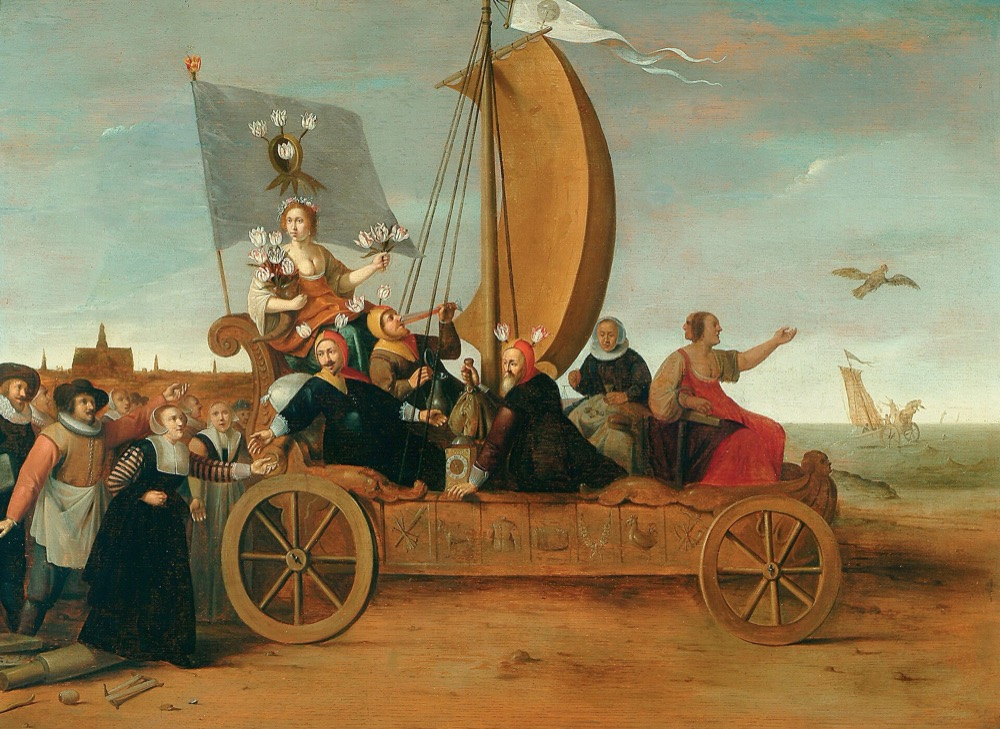
\includegraphics[height=0.36\textheight]{ch13_tulip_mania_1637.jpg}\\[1mm]
\imgcap{Carul nebunilor al Florei, c.~1637}
\imgcredit{https://commons.wikimedia.org/wiki/File:Flora's_Wagon_of_Fools_(Flora's_Mallewagen)_tulipomania,_Hendrik_Gerritsz_Pot_c1637.jpg}{Pictură: Hendrik Gerritsz Pot (c.~1637); domeniu public; Wikimedia Commons}
\end{column}
\begin{column}{0.6\textwidth}
\begin{itemize}
    \item \textbf{Mania lalelelor}, Olanda, 1636--1637: contracte pe bulbi rari tranzacționate la prețuri extreme, apoi prăbușite în februarie 1637
    \begin{itemize}
        \item \refGarber: o parte din poveste este mit; bulbii rari erau scumpi din motive întemeiate, bulbii obișnuiți arată mania
    \end{itemize}
    \item \textbf{South Sea} (1720), \textbf{Wall Street} (1929), \textbf{Japonia} (1989), \textbf{dot-com} (2000), \textbf{imobiliare} (2007), \textbf{cripto} (2017, 2021)
    \item Tiparul comun \refKA: o poveste nouă, credit ieftin, prețuri în creștere care atrag noi cumpărători, apoi panică
\end{itemize}
\end{column}
\end{columns}
\end{frame}

\begin{frame}{1929 și 1987}
\itemsize{\footnotesize}
\begin{columns}[T]
\begin{column}{0.38\textwidth}
\centering
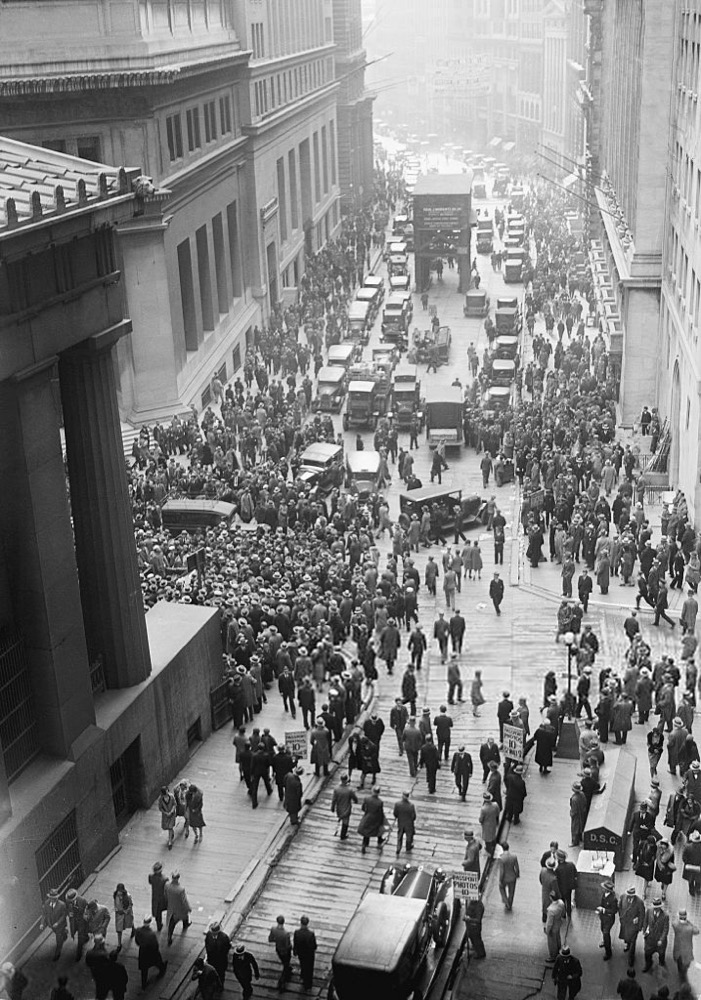
\includegraphics[height=0.42\textheight]{ch13_nyse_crowd_1929.jpg}\\[1mm]
\imgcap{Mulțime în fața Bursei din New York, 29 octombrie 1929}
\imgcredit{https://commons.wikimedia.org/wiki/File:Crowd_outside_nyse.jpg}{Foto: US government (1929); domeniu public; Wikimedia Commons}
\end{column}
\begin{column}{0.6\textwidth}
\begin{itemize}
    \item \textbf{Octombrie 1929}: sfîrșitul boom-ului anilor 1920 și începutul Marii Crize
    \item \textbf{19 octombrie 1987} (Black Monday): cea mai mare scădere într-o singură zi a indicelui Dow Jones, fără vreo știre majoră în acea zi
    \begin{itemize}
        \item \refSJB\ au găsit oscilații log-periodice, tot mai rapide, în anii dinaintea lui 1987; această observație a pornit literatura LPPL
        \item datele zilnice ale cursului încep în 1990: studiem 1987 prin literatură, iar bulele de mai tîrziu cu datele noastre
    \end{itemize}
    \item Un crah fără știri sugerează o cauză \textbf{endogenă}: piața însăși devenise fragilă
\end{itemize}\centering
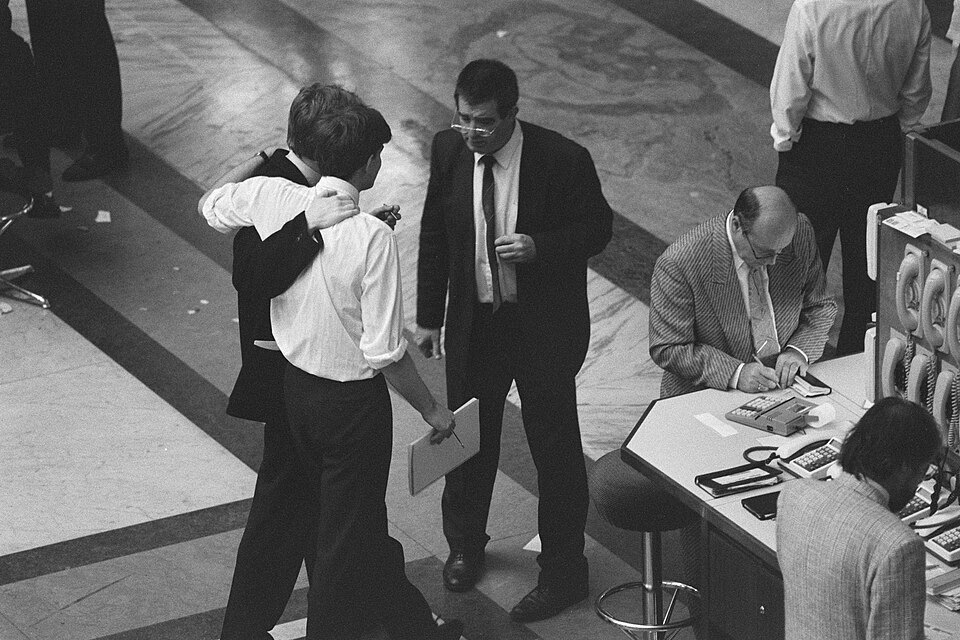
\includegraphics[height=0.17\textheight]{ch13_amsterdam_crash_1987.jpg}\\[1mm]
\imgcap{Bursa din Amsterdam, 21 octombrie 1987}
\imgcredit{https://commons.wikimedia.org/wiki/File:Effectenbeurs_Amsterdam_na_koersval,_Bestanddeelnr_934-1094.jpg}{Foto: Bart Molendijk / Anefo, Nationaal Archief (1987); CC0; Wikimedia Commons}
\end{column}
\end{columns}
\end{frame}

\begin{frame}{Valoarea fundamentală și bula}
\itemsize{\small}
\begin{itemize}
    \item \textbf{Valoarea fundamentală} $F_t$: valoarea actualizată a fluxurilor de numerar viitoare așteptate (dividendele $D$), actualizate cu rata $r$
    \begin{itemize}
        \item $F_t = \sum_{k=1}^{\infty} \dfrac{E_t[D_{t+k}]}{(1+r)^k}$
    \end{itemize}
    \item \textbf{Componenta de bulă}: $B_t = P_t - F_t$, partea din preț neexplicată de fundamente
    \begin{itemize}
        \item $F_t$ nu este observată: putem testa doar \textbf{implicațiile} unei bule asupra traiectoriei prețului
    \end{itemize}
    \item Două puncte de vedere
    \begin{itemize}
        \item piețe eficiente: prețurile reflectă informația; „bulele” se văd doar retrospectiv \refFama
        \item finanțe comportamentale: comportamentul de turmă și extrapolarea îndepărtează prețurile de valoare \refShiller; creșterile mari ridică probabilitatea unui crah \refGSY
    \end{itemize}
\end{itemize}
\end{frame}

\begin{frame}{Șase creșteri și crahuri în datele cursului}
\itemsize{\footnotesize}
\begin{center}
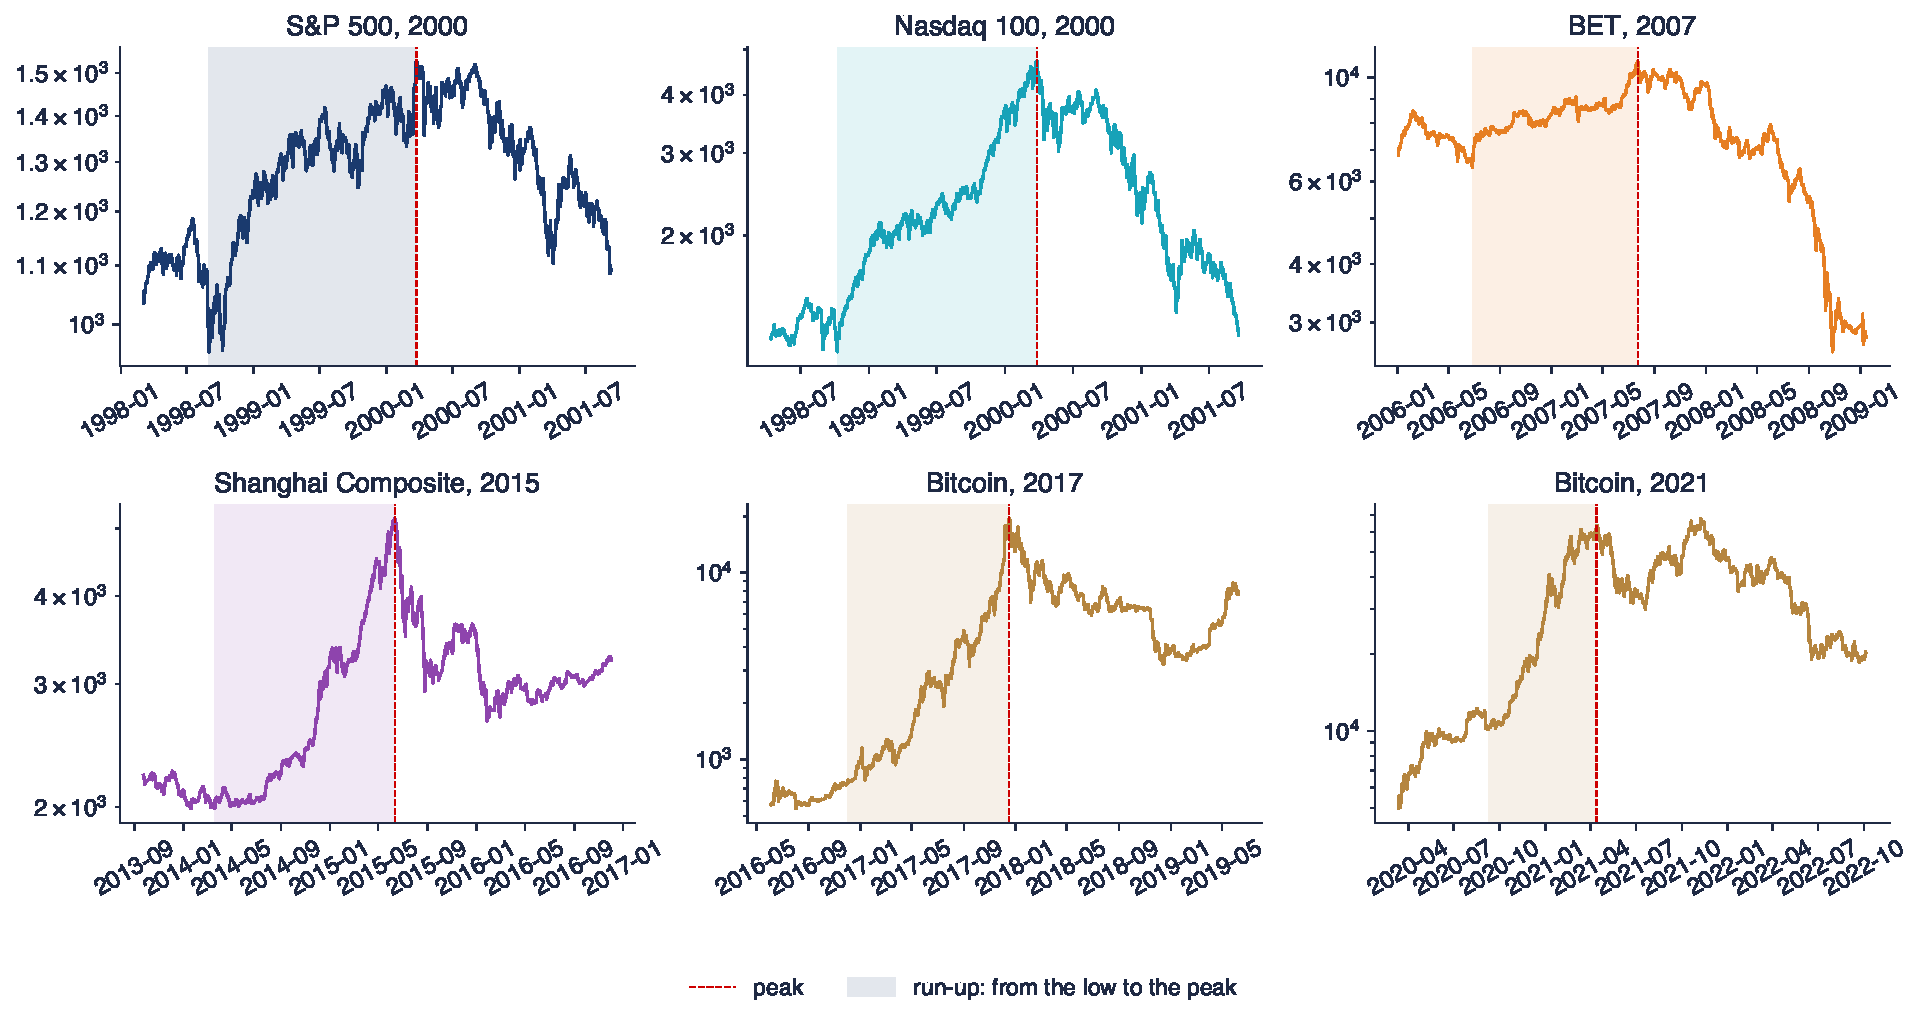
\includegraphics[width=0.97\textwidth,height=0.66\textheight,keepaspectratio]{tsa_ch13_episodes.pdf}
\end{center}
\vspace{-0.25cm}
\begin{itemize}
    \item Închideri zilnice, scară logaritmică, de la șase luni înainte de minimul creșterii pînă la optsprezece luni după maximum; zona colorată: creșterea de la minim la maximum
\end{itemize}
\quantlet{TSA\_ch13\_episodes}{\qlurl{TSA_ch13_episodes}}
\end{frame}

\begin{frame}{Interpretarea celor șase episoade}
\itemsize{\footnotesize}
\setlength{\tabcolsep}{4pt}\begin{center}
\scriptsize
\begin{tabular}{lllrrr}
\toprule
\textbf{Episodul} & \textbf{Minim} & \textbf{Maxim} & \textbf{Creștere} & \textbf{Ritm anual} & \textbf{Scădere în 1 an} \\
\midrule
S\&P 500, 2000 & 31 august 1998 & 24 martie 2000 & 60\% & 30\% & 27\% \\
Nasdaq 100, 2000 & 8 octombrie 1998 & 27 martie 2000 & 317\% & 97\% & 66\% \\
BET, 2007 & 27 iunie 2006 & 24 iulie 2007 & 68\% & 48\% & 50\% \\
Shanghai Composite, 2015 & 20 martie 2014 & 12 iunie 2015 & 159\% & 77\% & 49\% \\
Bitcoin, 2017 & 1 decembrie 2016 & 16 decembrie 2017 & 2476\% & 312\% & 83\% \\
Bitcoin, 2021 & 8 septembrie 2020 & 13 aprilie 2021 & 527\% & 309\% & 53\% \\
\bottomrule
\end{tabular}
\end{center}
\begin{itemize}
    \item Ritmul anual: $\ln(P_{\text{maxim}}/P_{\text{minim}})$ împărțit la durata creșterii în ani; scăderea: cea mai mică închidere din anul de după maximum, față de maximum
    \item Bitcoin și-a înmulțit prețul de 26 ori în aproximativ un an; S\&P 500 a crescut mult mai puțin: nu orice maximum este o bulă de aceeași intensitate
\end{itemize}
\end{frame}

\begin{frame}{Recapitulare: bule în istorie}
\itemsize{\small}
\begin{itemize}
    \item O bulă este un preț peste valoarea fundamentală $F_t$; $F_t$ nu este observată
    \item Șase episoade în datele noastre: creșteri între 60\% și 2476\%, urmate de scăderi între 27\% și 83\% într-un an
    \item Semnături: creștere explozivă și superexponențială, oscilații tot mai rapide, apoi un sfîrșit
\end{itemize}
\end{frame}


%=============================================================================
\section{Bule raționale și rădăcini explozive}
%=============================================================================

\begin{frame}{De ce o bulă rațională trebuie să explodeze}
\itemsize{\small}
\begin{itemize}
    \item Evaluarea fără arbitraj: $P_t = \dfrac{E_t[P_{t+1} + D_{t+1}]}{1+r}$; valoarea fundamentală $F_t$ este o soluție
    \begin{itemize}
        \item orice $P_t = F_t + B_t$ cu $E_t[B_{t+1}] = (1+r)\,B_t$ este tot o soluție
    \end{itemize}
    \item Bula trebuie să crească, în medie, cu rata $r$: $E_t[B_{t+k}] = (1+r)^k B_t$
    \begin{itemize}
        \item un investitor deține un activ peste valoarea lui doar dacă se așteaptă ca supraevaluarea să crească
        \item $1+r > 1$: componenta de bulă este un proces \textbf{exploziv}
    \end{itemize}
    \item Consecință: dacă dividendele sînt $I(1)$ (\tsachlink{https://danpele.github.io/Time-Series-Analysis/RO/Cursuri/capitol3_radacini_unitare_modele_arima.pdf}{Capitolul 3}), prețul este $I(1)$ fără bulă și exploziv cu bulă
\end{itemize}
\end{frame}

\begin{frame}{Exemplu rezolvat: o bulă care se poate sparge}
\itemsize{\small}
\begin{itemize}
    \item \refBW: în fiecare perioadă bula supraviețuiește cu probabilitatea $\pi$ și crește atunci la $\frac{1+r}{\pi}B_t$; altfel se sparge ($B_{t+1} \approx 0$)
    \begin{itemize}
        \item verificare: $E_t[B_{t+1}] = \pi \cdot \frac{1+r}{\pi} B_t + (1-\pi) \cdot 0 = (1+r)B_t$
    \end{itemize}
    \item Cu $r = 2\%$ și $\pi = 0{,}98$ pe perioadă:
    \begin{itemize}
        \item cît supraviețuiește, bula crește cu $1{,}02/0{,}98 - 1 = 4{,}08\%$ pe perioadă, mai mult decît $r$: creșterea suplimentară plătește riscul spargerii
        \item durata medie de viață $1/(1-\pi) = 50$ de perioade; supraviețuiește peste 34 de perioade cu probabilitatea $1/2$ ($0{,}98^{k} = 0{,}5$)
    \end{itemize}
    \item Cu cît bula durează mai mult, cu atît trebuie să crească mai repede și cu atît este mai mare căderea la spargere
\end{itemize}
\end{frame}

\begin{frame}{O bulă rațională simulată și trei rădăcini AR(1)}
\itemsize{\footnotesize}
\begin{center}
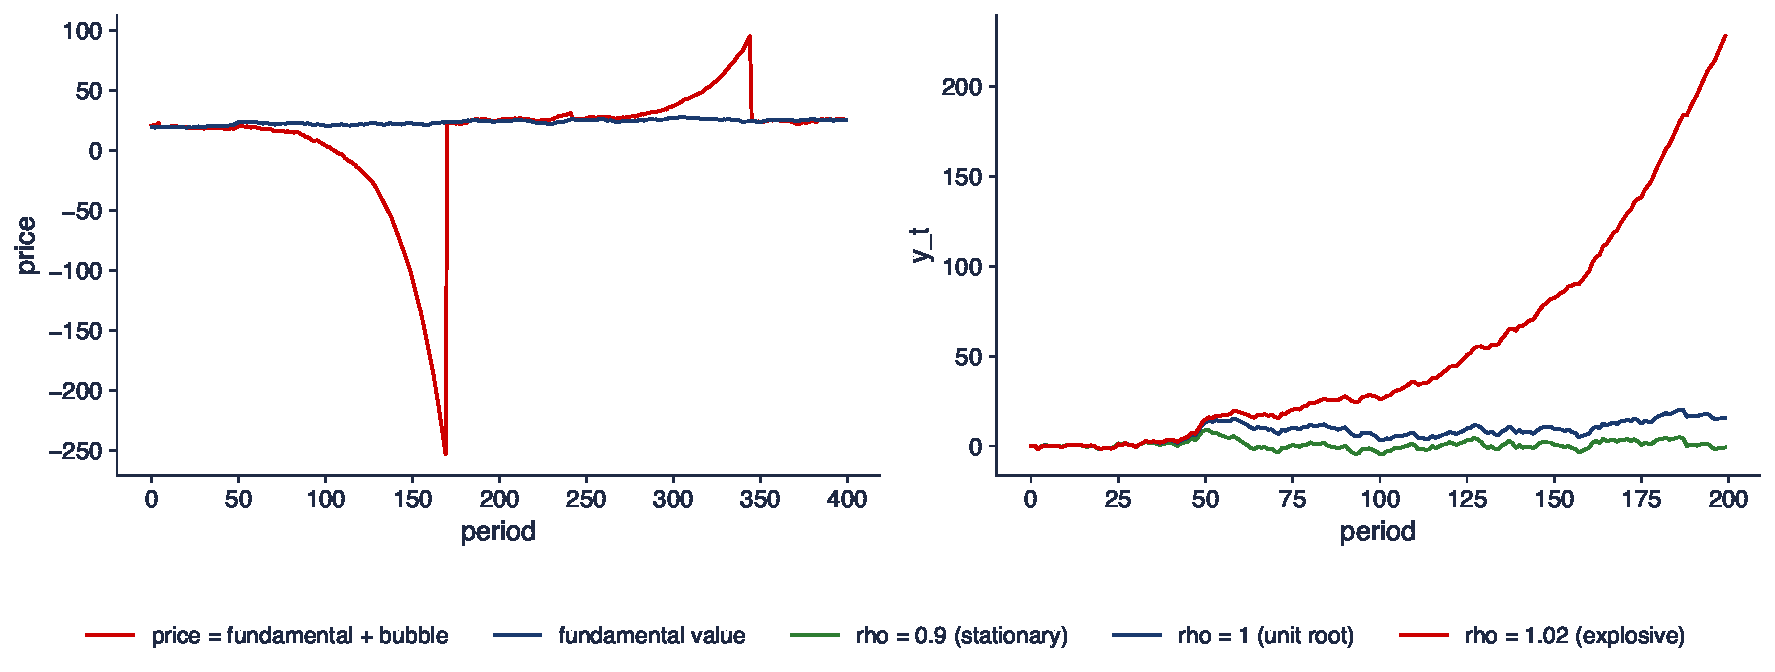
\includegraphics[width=0.97\textwidth,height=0.6\textheight,keepaspectratio]{tsa_ch13_rational.pdf}
\end{center}
\vspace{-0.25cm}
\begin{itemize}
    \item Stînga: valoarea fundamentală (mers aleator) plus o bulă Blanchard--Watson ($r = 2\%$, $\pi = 0{,}98$), 400 de perioade; dreapta: $y_t = \rho y_{t-1} + \varepsilon_t$ cu aceleași șocuri și $\rho = 0{,}9$, $1$, $1{,}02$
\end{itemize}
\quantlet{TSA\_ch13\_rational\_bubble}{\qlurl{TSA_ch13_rational_bubble}}
\end{frame}

\begin{frame}{Interpretarea simulării}
\itemsize{\small}
\begin{itemize}
    \item Bula crește, se sparge, reîncepe: pe această traiectorie atinge 71 și se sparge de 2 ori după ce a devenit mare
    \begin{itemize}
        \item prețul preia episoadele explozive; între ele urmează valoarea fundamentală
    \end{itemize}
    \item Rădăcinile AR(1) (\tsachlink{https://danpele.github.io/Time-Series-Analysis/RO/Cursuri/capitol3_radacini_unitare_modele_arima.pdf}{Capitolul 3}): $\rho = 0{,}9$ revine la medie, $\rho = 1$ rătăcește (rădăcină unitară), $\rho = 1{,}02$ explodează
    \begin{itemize}
        \item cu $\rho = 1{,}02$ un șoc se dublează în aproximativ 35 de perioade și se înmulțește cu 7{,}24 după 100
    \end{itemize}
    \item Ideea testelor: o rădăcină explozivă ($\rho > 1$) în prețul logaritmic în timpul unei creșteri este urma statistică a unei bule raționale
\end{itemize}
\end{frame}

\begin{frame}{Teste de rădăcină unitară la dreapta}
\itemsize{\small}
\begin{itemize}
    \item Regresia din \tsachlink{https://danpele.github.io/Time-Series-Analysis/RO/Cursuri/capitol3_radacini_unitare_modele_arima.pdf}{Capitolul 3} pe o fereastră a prețului logaritmic $y_t = \ln P_t$: $\Delta y_t = a + \delta\, y_{t-1} + \varepsilon_t$, cu $\delta = \rho - 1$
    \begin{itemize}
        \item \tsachlink{https://danpele.github.io/Time-Series-Analysis/RO/Cursuri/capitol3_radacini_unitare_modele_arima.pdf}{Capitolul 3} (\refDF): $H_0$: $\delta = 0$ față de $H_1$: $\delta < 0$ (staționar), coada din \textbf{stînga}
        \item bule: $H_0$: $\delta = 0$ (rădăcină unitară) față de $H_1$: $\delta > 0$ (exploziv), coada din \textbf{dreapta}: respingem pentru statistici $t$ mari
    \end{itemize}
    \item Problema: o bulă ocupă doar o parte din eșantion, iar crahul de după ea seamănă cu revenirea la medie
    \begin{itemize}
        \item un singur test ADF pe tot eșantionul nu are aproape nicio putere: trebuie să calculăm testul pe multe \textbf{ferestre}
    \end{itemize}
    \item Notații: $r_1, r_2 \in [0,1]$ sînt fracțiuni din eșantion; $\mathrm{ADF}_{r_1}^{r_2}$ este statistica $t$ a lui $\hat\delta$ pe fereastra de la $r_1T$ la $r_2T$; $r_0$ este cea mai mică fereastră
\end{itemize}
\end{frame}

\begin{frame}{SADF, GSADF și BSADF}
\itemsize{\small}
\begin{itemize}
    \item \textbf{SADF} \refPWY: început fixat la 0, sfîrșitul înaintează: $\mathrm{SADF} = \sup_{r_2 \in [r_0, 1]} \mathrm{ADF}_{0}^{r_2}$
    \begin{itemize}
        \item bun pentru o singură bulă; după un prim crah își pierde puterea
    \end{itemize}
    \item \textbf{GSADF} \refPSYa: se mișcă și începutul, și sfîrșitul: $\mathrm{GSADF} = \sup_{r_2 \in [r_0,1]}\ \sup_{r_1 \in [0, r_2 - r_0]} \mathrm{ADF}_{r_1}^{r_2}$
    \begin{itemize}
        \item detectează mai multe bule într-un eșantion; fereastra minimă $r_0 = 0{,}01 + 1{,}8/\sqrt{T}$
    \end{itemize}
    \item \textbf{BSADF} (datarea): pentru fiecare dată $r_2$, $\mathrm{BSADF}(r_2) = \sup_{r_1} \mathrm{ADF}_{r_1}^{r_2}$, folosind doar datele pînă la $r_2$
    \begin{itemize}
        \item un episod începe cînd BSADF depășește valoarea critică și durează cel puțin $\log T$ observații \refPSYb
    \end{itemize}
    \item Distribuțiile nu sînt standard: valorile critice se obțin prin Monte Carlo, sub un mers aleator cu drift slab, $y_t = T^{-1} + y_{t-1} + \varepsilon_t$
\end{itemize}
\end{frame}

\begin{frame}{Exemplu rezolvat: o fereastră din Nasdaq 100}
\itemsize{\small}
\begin{itemize}
    \item Închideri săptămînale logaritmice ale Nasdaq 100, $T = 782$ de săptămîni; $r_0 = 0{,}074$, adică o fereastră minimă de 58 de săptămîni
    \begin{itemize}
        \item sfîrșitul ferestrei: 24 martie 2000, săptămîna maximului; dintre toate punctele de început, cea mai mare statistică provine din începutul 17 ianuarie 1992
    \end{itemize}
    \item OLS pe această fereastră ($n = 427$ de variații săptămînale): $\widehat{\Delta y_t} = -0{,}0336 + 0{,}0060\, y_{t-1}$
    \begin{itemize}
        \item $t = \hat\delta / \mathrm{SE}(\hat\delta) = 0{,}0060 / 0{,}0021 = 2{,}91$
        \item deci BSADF la maximum este 2{,}91, peste valoarea critică de 95\%, egală cu 0{,}54
    \end{itemize}
    \item Lectura: $\hat\delta > 0$ înseamnă $\hat\rho = 1 + \hat\delta > 1$: cu cît prețul este mai mare, cu atît creșterea săptămînală următoare este mai mare, semnul unei faze explozive
\end{itemize}
\end{frame}

\begin{frame}{Episoadele explozive ale Nasdaq 100, 1990--2004}
\itemsize{\footnotesize}
\begin{center}
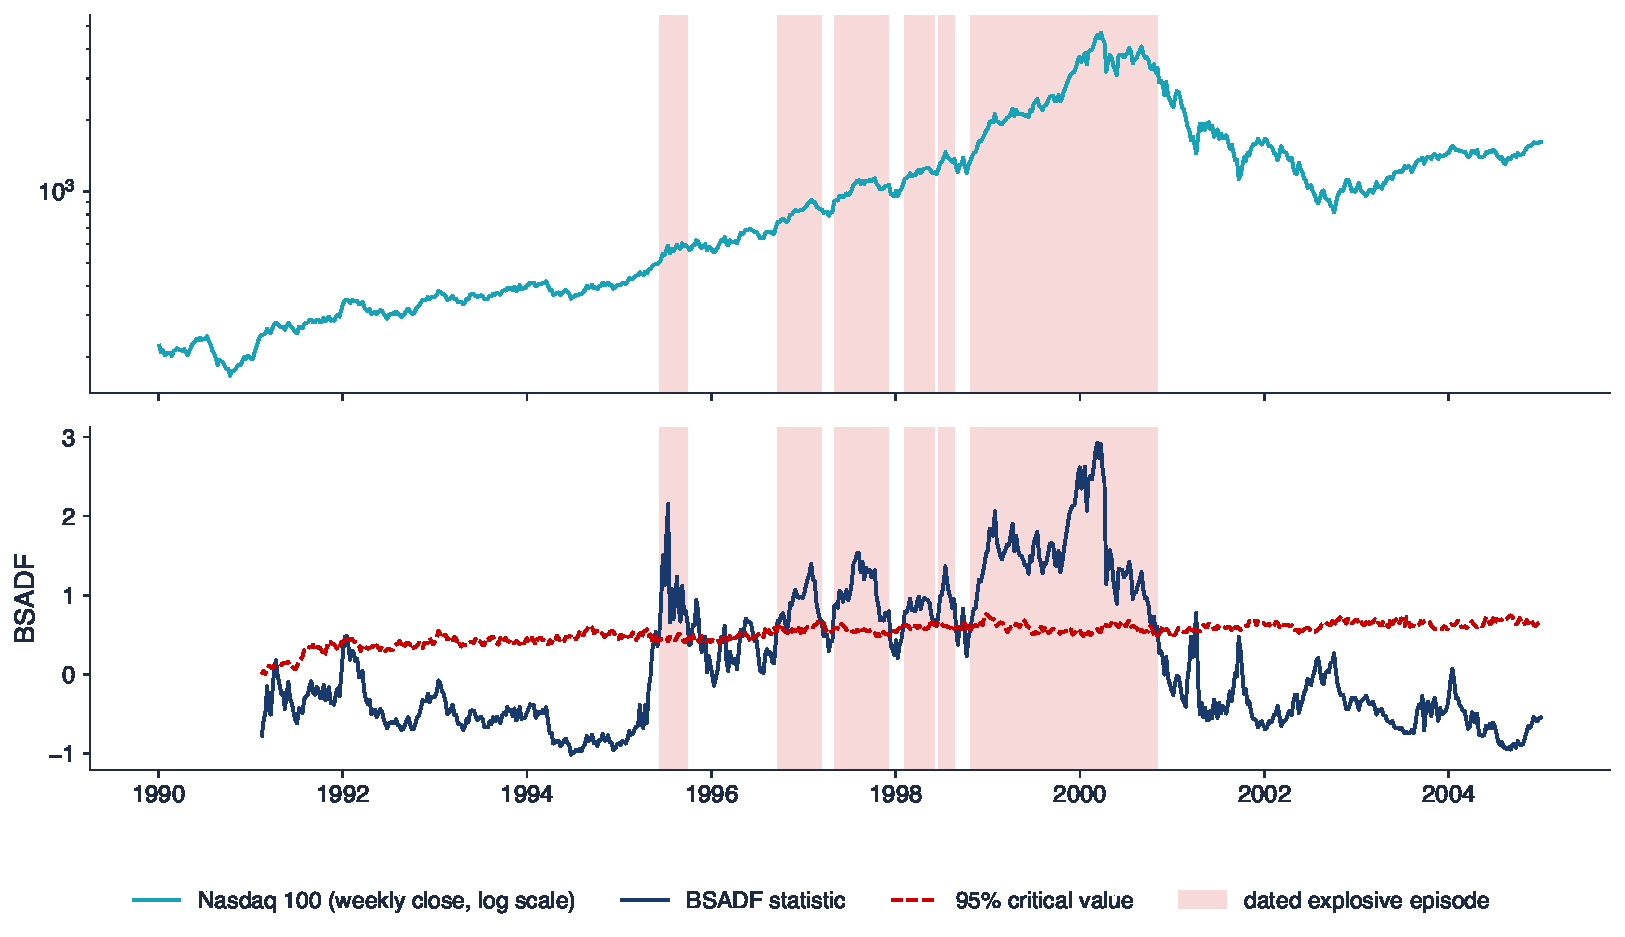
\includegraphics[width=0.97\textwidth,height=0.62\textheight,keepaspectratio]{tsa_ch13_psy_ndx.pdf}
\end{center}
\vspace{-0.25cm}
\begin{itemize}
    \item Sus: închiderea săptămînală, scară logaritmică; jos: BSADF și valorile critice de 95\% (Monte Carlo, 1000 de mersuri aleatoare); zone colorate: episoadele datate (cel puțin 7 săptămîni peste valoarea critică)
\end{itemize}
\quantlet{TSA\_ch13\_explosive\_roots}{\qlurl{TSA_ch13_explosive_roots}}
\end{frame}

\begin{frame}{Interpretarea testelor pentru Nasdaq 100}
\itemsize{\small}
\begin{itemize}
    \item ADF pe tot eșantionul $-1{,}27$ (valoarea critică de 95\%: $-0{,}13$): nicio dovadă; SADF 2{,}72 (1{,}48) și GSADF 2{,}92 (2{,}28): comportament exploziv
    \begin{itemize}
        \item crahul din 2000--2002 ascunde bula de un test unic pe tot eșantionul
    \end{itemize}
    \item BSADF datează 6 episoade; cel mai lung ține de la 23 octombrie 1998 pînă la 3 noiembrie 2000 (107 săptămîni)
    \begin{itemize}
        \item episoade explozive scurte încă din iunie 1995: boom-ul anilor 1990 a venit în valuri, cum au găsit \refPWY
    \end{itemize}
    \item Data de sfîrșit este tîrzie: statistica rămîne mare luni de zile după maximum; testul datează exuberanța, nu anunță crahul
\end{itemize}
\end{frame}

\begin{frame}{Bitcoin, BET și Shanghai: episoade datate}
\itemsize{\footnotesize}
\begin{center}
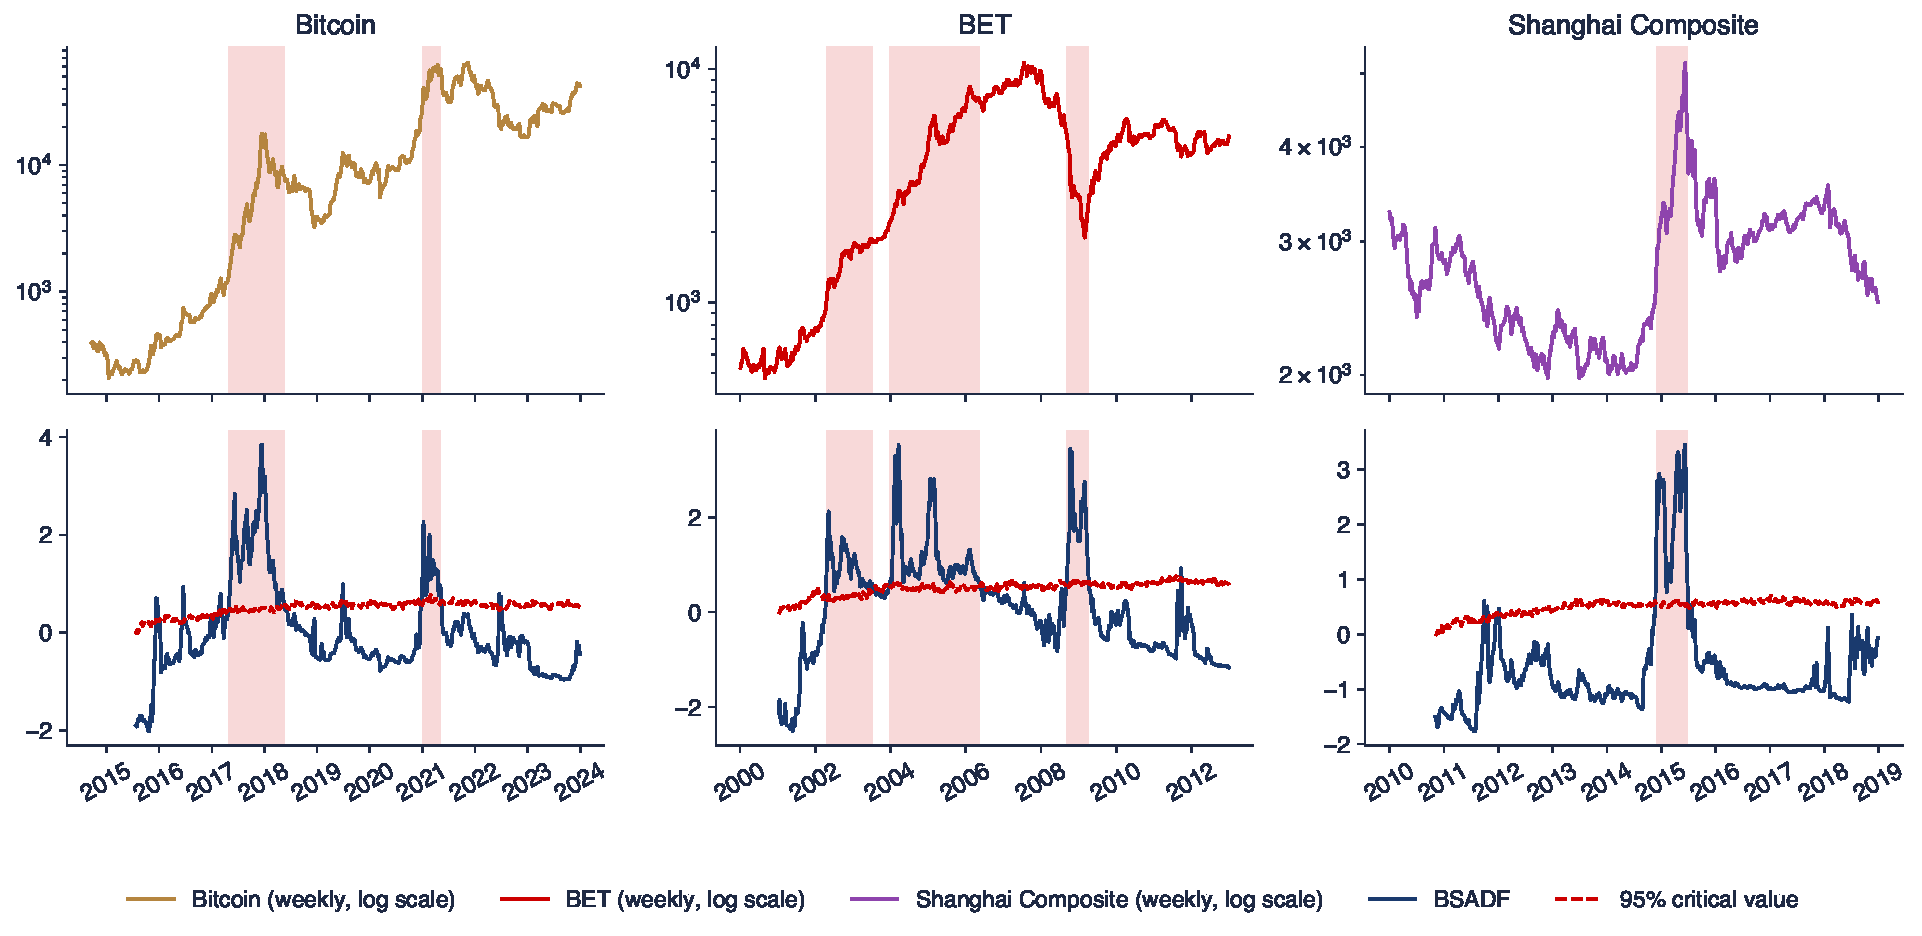
\includegraphics[width=0.97\textwidth,height=0.62\textheight,keepaspectratio]{tsa_ch13_psy_panel.pdf}
\end{center}
\vspace{-0.25cm}
\begin{itemize}
    \item Închideri săptămînale logaritmice; sus: prețul cu episoadele datate; jos: BSADF și valorile critice de 95\%; Bitcoin 2014--2023, BET 2000--2012, Shanghai Composite 2010--2018
\end{itemize}
\quantlet{TSA\_ch13\_explosive\_roots}{\qlurl{TSA_ch13_explosive_roots}}
\end{frame}

\begin{frame}{Interpretarea celor trei piețe}
\itemsize{\small}
\begin{itemize}
    \item GSADF: Bitcoin 3{,}85, BET 3{,}53, Shanghai 3{,}46; toate peste valorile critice de 95\% (aproximativ 2{,}18)
    \begin{itemize}
        \item Bitcoin: aprilie 2017 -- mai 2018 și ianuarie 2021 -- mai 2021; Shanghai: noiembrie 2014 -- iunie 2015
    \end{itemize}
    \item BET: faza explozivă este decembrie 2003 -- mai 2006, nu creșterea pînă în iulie 2007, care a fost puternică, dar nu explozivă
    \begin{itemize}
        \item semnalul BET din septembrie 2008 -- aprilie 2009 este prăbușirea: o \textbf{scădere care se accelerează} dă tot $\hat\delta > 0$; citiți întotdeauna datele alături de graficul prețului
    \end{itemize}
    \item Episodul Bitcoin din 2017 ține pînă în mai 2018, din nou mult după maximum
\end{itemize}
\end{frame}

\begin{frame}{Limitele testelor de rădăcini explozive}
\itemsize{\small}
\begin{itemize}
    \item \textbf{Fundamentele}: un preț exploziv este bulă doar dacă fundamentele nu sînt explozive
    \begin{itemize}
        \item mai bine: testați raportul preț--dividend (\refPSYa\ pentru S\&P 500); pentru Bitcoin nu există deloc dividende
    \end{itemize}
    \item \textbf{Volatilitatea}: volatilitatea variabilă distorsionează nivelul testului; un wild bootstrap dă valori critice robuste \refPS
    \item \textbf{Momentul}: BSADF folosește doar date trecute, deci poate rula în timp real; dar semnalează o bulă deja în desfășurare și nu spune nimic despre momentul în care se termină
    \begin{itemize}
        \item modelul LPPL din secțiunea următoare încearcă să răspundă exact la această întrebare: cînd?
    \end{itemize}
\end{itemize}
\end{frame}

\begin{frame}{Recapitulare: bule raționale și rădăcini explozive}
\itemsize{\small}
\begin{itemize}
    \item O bulă rațională crește în medie cu rata $r$: $E_t[B_{t+1}] = (1+r)B_t$, un proces exploziv
    \item ADF la dreapta: $H_1$: $\delta > 0$; SADF și GSADF iau supremumul pe ferestre; BSADF datează episoadele
    \item Nasdaq 100, Bitcoin, BET și Shanghai au episoade explozive; testele datează creșterea, nu crahul
\end{itemize}
\end{frame}


%=============================================================================
\section{Modelul LPPL}
%=============================================================================

\begin{frame}{Crahurile ca puncte critice}
\itemsize{\footnotesize}
\begin{columns}[T]
\begin{column}{0.38\textwidth}
\centering
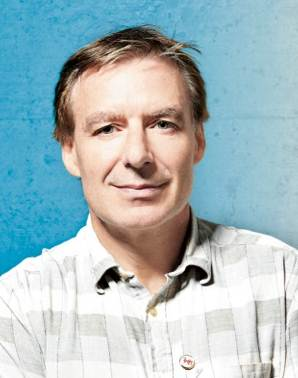
\includegraphics[height=0.36\textheight]{ch13_sornette_2012.jpg}\\[1mm]
\imgcap{Didier Sornette (n.~1957)}
\imgcredit{https://commons.wikimedia.org/wiki/File:Didier_Sornette.jpg}{Foto: Didier Sornette (2012); CC BY-SA 3.0 DE; Wikimedia Commons}
\end{column}
\begin{column}{0.6\textwidth}
\begin{itemize}
    \item Fizician, ETH Zürich; împreună cu Anders Johansen și Olivier Ledoit a propus \textbf{modelul JLS} \refJLS
    \item Ideea: investitorii își imită vecinii; imitația creează o reacție pozitivă (positive feedback)
    \begin{itemize}
        \item prețurile în creștere atrag cumpărători, care urcă prețurile și mai mult: creșterea se accelerează
        \item piața devine tot mai fragilă, ca un sistem fizic aproape de un \textbf{punct critic} (apa aproape de fierbere)
    \end{itemize}
    \item \textbf{Timpul critic} $t_c$: momentul cel mai probabil al sfîrșitului bulei
    \begin{itemize}
        \item un crah este probabil aproape de $t_c$, dar nu sigur: bula se poate încheia și cu o scădere lentă
    \end{itemize}
\end{itemize}
\end{column}
\end{columns}
\end{frame}

\begin{frame}{Creșterea superexponențială}
\itemsize{\small}
\begin{itemize}
    \item Creșterea \textbf{exponențială}: ritm de creștere constant, $\ln P(t) = a + g\,t$; $d \ln P/dt = g$
    \begin{itemize}
        \item o dreaptă pe scară logaritmică
    \end{itemize}
    \item Creșterea \textbf{superexponențială}: ritmul de creștere crește în timp; pe scară logaritmică curba se îndoaie în sus
    \begin{itemize}
        \item singularitate de tip lege de putere: $\ln P(t) = A + B\,(t_c - t)^m$, cu $B < 0$ și $0 < m < 1$
        \item ritmul de creștere $d \ln P/dt = -Bm\,(t_c - t)^{m-1} \to \infty$ cînd $t \to t_c$, în timp ce $\ln P(t_c) = A$ rămîne finit
    \end{itemize}
    \item O astfel de creștere nu poate dura: trebuie să se încheie la $t_c$ sau înainte, o \textbf{singularitate în timp finit}
\end{itemize}
\end{frame}

\begin{frame}{Creștere exponențială și creștere superexponențială}
\itemsize{\footnotesize}
\begin{center}
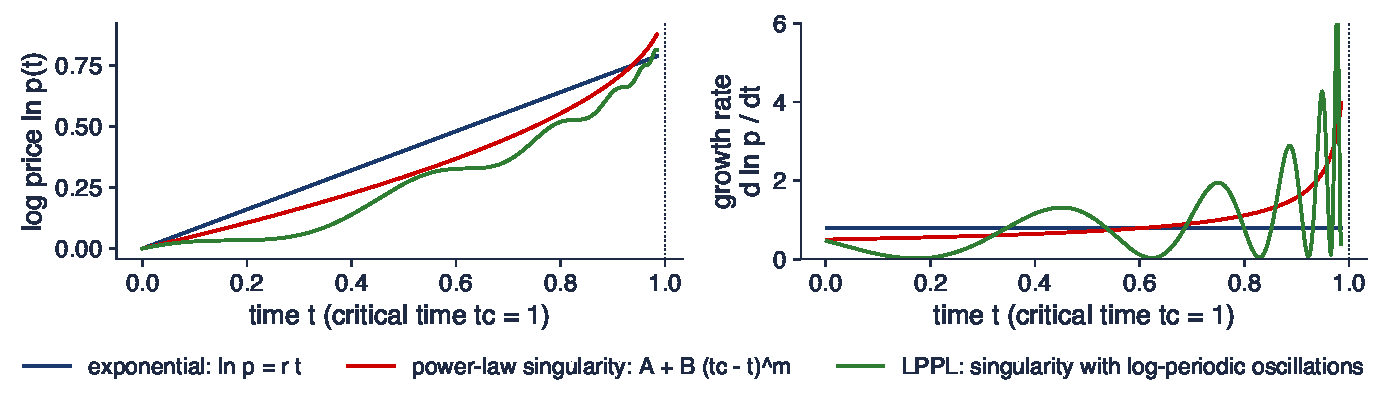
\includegraphics[width=0.97\textwidth,height=0.58\textheight,keepaspectratio]{tsa_ch13_growth.pdf}
\end{center}
\vspace{-0.25cm}
\begin{itemize}
    \item Stînga: prețul logaritmic; dreapta: ritmul lui de creștere $d \ln p/dt$; exponențială ($r = 0{,}8$), singularitate de tip lege de putere ($A = 1$, $B = -1$, $m = 0{,}5$, $t_c = 1$) și aceeași cu oscilații log-periodice
\end{itemize}
\quantlet{TSA\_ch13\_lppl\_model}{\qlurl{TSA_ch13_lppl_model}}
\end{frame}

\begin{frame}{Interpretarea traiectoriilor de creștere}
\itemsize{\small}
\begin{itemize}
    \item Toate trei încep cu ritmuri de creștere asemănătoare: la începutul unei bule traiectoriile se disting greu
    \item Ritmul exponențial rămîne 0,8; ritmul singular crește de la 0{,}50 la 0{,}70 la jumătatea drumului și la 3{,}98 chiar înainte de $t_c$
    \item Oscilațiile se suprapun peste trendul accelerat și devin mai rapide aproape de $t_c$: slide-urile următoare explică de ce
\end{itemize}
\end{frame}

\begin{frame}{De la riscul de crah la ecuația LPPL}
\itemsize{\footnotesize}
\begin{itemize}
    \item JLS: înainte de crah, $dP/P = \mu(t)\,dt + \sigma\,dW - \kappa\, dj$; $j$ sare de la 0 la 1 la crah, care elimină o fracțiune $\kappa$ din preț
    \begin{itemize}
        \item \textbf{rata de hazard} $h(t)$: probabilitatea pe unitatea de timp ca crahul să aibă loc acum, știind că nu a avut loc pînă acum
    \end{itemize}
    \item Fără arbitraj: $E[dP] = 0$ $\Rightarrow$ $\mu(t) = \kappa\, h(t)$: prețul trebuie să crească pentru a-i plăti pe investitori pentru riscul de crah
    \begin{itemize}
        \item cu cît hazardul este mai mare, cu atît prețul trebuie să crească mai repede: riscul și creșterea cresc împreună
    \end{itemize}
    \item Imitația aproape de un punct critic dă $h(t) \approx \alpha (t_c - t)^{m-1}[1 + \beta\cos(\omega \ln(t_c - t) - \phi')]$
    \begin{itemize}
        \item integrînd $\mu(t) = \kappa h(t)$ în timp obținem prețul logaritmic de pe slide-ul următor
    \end{itemize}
\end{itemize}
\end{frame}

\begin{frame}{Ecuația LPPL}
\itemsize{\footnotesize}
\begin{itemize}
    \item \textbf{Legea de putere log-periodică} (LPPL), pentru $t < t_c$: $\quad \ln P(t) = A + B\,(t_c - t)^m + C\,(t_c - t)^m \cos\bigl(\omega \ln(t_c - t) - \phi\bigr)$
\end{itemize}\begin{center}
\scriptsize
\begin{tabular}{lll}
\toprule
\textbf{Parametrul} & \textbf{Semnificația} & \textbf{Interval uzual} \\
\midrule
$t_c$ & timpul critic: sfîrșitul cel mai probabil al bulei & după ultima observație \\
$A$ & prețul logaritmic la $t_c$ (dacă bula ar atinge $t_c$) & $A > 0$ \\
$B$ & mărimea creșterii de tip lege de putere & $B < 0$ (preț în creștere) \\
$m$ & exponentul: cît de repede se accelerează creșterea & $0 < m < 1$ \\
$C$ & mărimea relativă a oscilațiilor & $|C| < |B|$ \\
$\omega$ & frecvența unghiulară logaritmică a oscilațiilor & $2 \le \omega \le 25$ \\
$\phi$ & faza oscilațiilor & $[0, 2\pi)$ \\
\bottomrule
\end{tabular}
\end{center}
\begin{itemize}
    \item Șapte parametri: trei dintre ei ($t_c$, $m$, $\omega$) intră neliniar; $\phi$ dispare la estimare (Secțiunea 4)
\end{itemize}
\end{frame}

\begin{frame}{Oscilațiile log-periodice}
\itemsize{\small}
\begin{itemize}
    \item $\cos(\omega \ln(t_c - t) - \phi)$ este periodic în $\ln(t_c - t)$, nu în $t$: un ciclu complet de fiecare dată cînd $\ln(t_c - t)$ se schimbă cu $2\pi/\omega$
    \begin{itemize}
        \item maximele succesive $t_n$ verifică $\dfrac{t_c - t_n}{t_c - t_{n+1}} = \lambda = e^{2\pi/\omega}$: timpul rămas pînă la $t_c$ se micșorează cu același factor la fiecare ciclu
    \end{itemize}
    \item \textbf{Invarianța discretă la scală}: tiparul arată la fel cînd timpul pînă la $t_c$ se rescalează cu $\lambda$ (ca într-o ierarhie de investitori, grupuri, instituții)
    \item Exemplu rezolvat: pentru $\omega = 8$, $\lambda = e^{2\pi/8} = 2{,}19$
    \begin{itemize}
        \item dacă o corecție are loc cu 200 de zile înainte de $t_c$, următoarea vine cu aproximativ $200/2{,}19 \approx 91$ de zile înainte de $t_c$, apoi cu aproximativ 42, apoi 19
        \item $\omega = 6{,}28$ dă $\lambda = 2{,}72$; $\omega = 10$ dă $\lambda = 1{,}87$; literatura empirică raportează $\lambda$ în jur de 2 \refSornette
    \end{itemize}
\end{itemize}
\end{frame}

\begin{frame}{Componentele ecuației LPPL}
\itemsize{\footnotesize}
\begin{center}
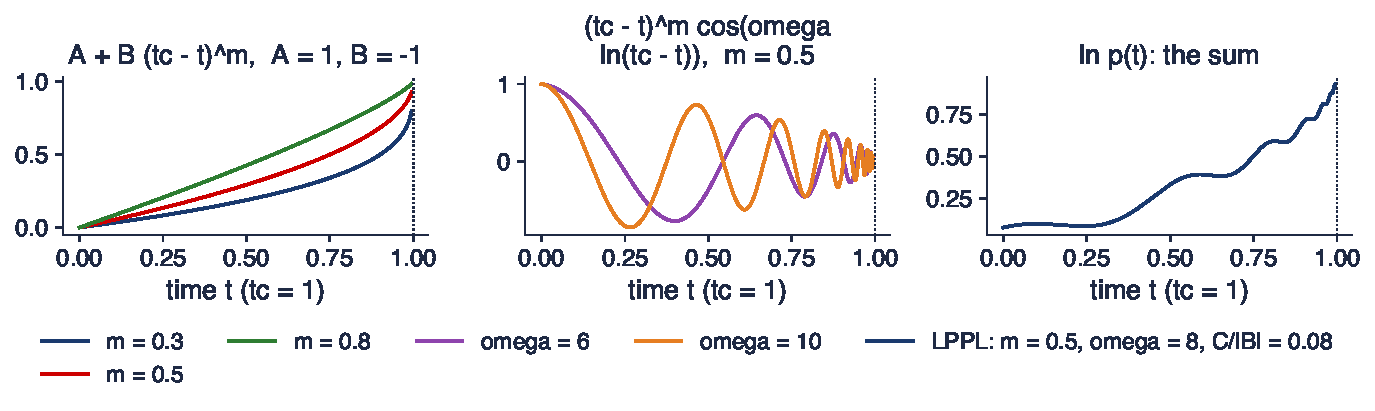
\includegraphics[width=0.97\textwidth,height=0.55\textheight,keepaspectratio]{tsa_ch13_lppl_components.pdf}
\end{center}
\vspace{-0.25cm}
\begin{itemize}
    \item Stînga: $A + B(t_c - t)^m$ pentru $m = 0{,}3;\ 0{,}5;\ 0{,}8$; mijloc: oscilația $(t_c - t)^m \cos(\omega \ln(t_c - t))$ pentru $\omega = 6$ și $10$; dreapta: traiectoria LPPL completă; $t_c = 1$
\end{itemize}
\quantlet{TSA\_ch13\_lppl\_model}{\qlurl{TSA_ch13_lppl_model}}
\end{frame}

\begin{frame}{Interpretarea componentelor}
\itemsize{\small}
\begin{itemize}
    \item Un $m$ mai mic concentrează creșterea aproape de $t_c$: curba este plată multă vreme, apoi urcă brusc
    \begin{itemize}
        \item $m$ apropiat de 1 este aproape o dreaptă: cu greu o bulă; $m$ apropiat de 0 este un salt la $t_c$
    \end{itemize}
    \item Termenul oscilant se micșorează cu $(t_c - t)^m$ și se accelerează: ciclurile se scurtează cu factorul $\lambda$
    \begin{itemize}
        \item un $\omega$ mai mare dă mai multe cicluri înainte de $t_c$
    \end{itemize}
    \item Creșterile reale (Secțiunea 4) arată acest amestec: un trend accelerat cu corecții tot mai dese
\end{itemize}
\end{frame}

\begin{frame}{Exemplu rezolvat: o valoare LPPL calculată de mînă}
\itemsize{\footnotesize}
\begin{itemize}
    \item Parametri: $A = 8$, $B = -1{,}2$, $C = 0{,}08$, $m = 0{,}5$, $\omega = 8$, $\phi = 0$, $t_c = 2$ (ani); calculați $\ln P(t)$
    \begin{itemize}
        \item $t = 1$: $t_c - t = 1$, $(t_c - t)^m = 1$, $\ln 1 = 0$, $\cos 0 = 1$: $\ln P = 8 - 1{,}2 + 0{,}08 = 6{,}880$, $P = 973$
        \item $t = 1{,}75$: $(0{,}25)^{0{,}5} = 0{,}500$, $\ln 0{,}25 = -1{,}386$, $\cos(8 \cdot (-1{,}386)) = 0{,}095$: $\ln P = 8 - 1{,}2 \cdot 0{,}500 + 0{,}08 \cdot 0{,}500 \cdot 0{,}095 = 7{,}404$, $P = 1642$
        \item $t = 1{,}99$: $(0{,}01)^{0{,}5} = 0{,}100$, $\cos(8 \cdot (-4{,}605)) = 0{,}654$: $\ln P = 7{,}885$, $P = 2658$
    \end{itemize}
    \item Prețul crește de la 973 la 2658 cînd $t$ trece de la 1 la 1,99 și ar atinge $e^A = 2981$ la $t_c$; cea mai mare parte a creșterii vine în ultimele luni
\end{itemize}
\end{frame}

\begin{frame}{Restricțiile parametrilor: filtrul}
\itemsize{\footnotesize}
\begin{itemize}
    \item O ajustare este \textbf{calificată} doar dacă descrie o bulă credibilă (\refSZ, după \refShanghai):
    \begin{itemize}
        \item $B < 0$: preț în creștere; $0{,}01 \le m \le 0{,}99$: creștere accelerată, cu preț finit la $t_c$
        \item $2 \le \omega \le 25$: oscilații nici prea lente, nici prea rapide; cel puțin 2,5 oscilații în fereastră, $\frac{\omega}{\pi}\ln\frac{t_c - t_1}{t_c - t_2} \ge 2{,}5$
        \item $t_2 \le t_c \le t_2 + 0{,}2\,(t_2 - t_1)$: sfîrșitul este aproape, raportat la lungimea ferestrei $[t_1, t_2]$
        \item amortizarea $\dfrac{m|B|}{\omega|C|} \ge 1$: rata de hazard rămîne pozitivă
    \end{itemize}
    \item Condiții asupra reziduurilor
    \begin{itemize}
        \item fiecare preț ajustat la cel mult 15\% de prețul observat; periodograma Lomb \refLomb\ confirmă ciclul log-periodic (nivel 10\%)
        \item reziduurile sînt staționare: testele Dickey--Fuller și Phillips--Perron din \tsachlink{https://danpele.github.io/Time-Series-Analysis/RO/Cursuri/capitol3_radacini_unitare_modele_arima.pdf}{Capitolul 3} resping rădăcina unitară (nivel 10\%)
    \end{itemize}
\end{itemize}
\end{frame}

\begin{frame}{Recapitulare: modelul LPPL}
\itemsize{\small}
\begin{itemize}
    \item Imitația creează o rată de hazard care crește spre $t_c$; lipsa arbitrajului o transformă în creștere superexponențială
    \item $\ln P(t) = A + B(t_c - t)^m + C(t_c - t)^m\cos(\omega\ln(t_c - t) - \phi)$, șapte parametri
    \item Log-periodic: ciclurile se scurtează cu $\lambda = e^{2\pi/\omega}$; o ajustare contează doar dacă trece de filtru
\end{itemize}
\end{frame}


%=============================================================================
\section{Estimarea}
%=============================================================================

\begin{frame}{Metoda în doi pași a lui Filimonov și Sornette}
\itemsize{\footnotesize}
\begin{itemize}
    \item Cele mai mici pătrate după șapte parametri, $\min \mathrm{SSR} = \sum_{t=t_1}^{t_2} [\ln P_t - \mathrm{LPPL}(t)]^2$, au multe minime locale; \refFS\ reduc căutarea la trei parametri
    \item Desfacem cosinusul: $C\cos(\omega\ln\tau - \phi) = C_1\cos(\omega\ln\tau) + C_2\sin(\omega\ln\tau)$, cu $\tau = t_c - t$, $C_1 = C\cos\phi$, $C_2 = C\sin\phi$
    \begin{itemize}
        \item $\ln P(t) = A + B\,f_t + C_1\,g_t + C_2\,h_t$ cu $f_t = \tau^m$, $g_t = \tau^m\cos(\omega\ln\tau)$, $h_t = \tau^m\sin(\omega\ln\tau)$
    \end{itemize}
    \item \textbf{Pasul 1} (liniar): pentru $(t_c, m, \omega)$ dați, regresăm $\ln P_t$ pe $(1, f_t, g_t, h_t)$ prin OLS: $(\hat A, \hat B, \hat C_1, \hat C_2) = (X'X)^{-1}X'y$
    \begin{itemize}
        \item obținem astfel costul concentrat $\mathrm{SSR}(t_c, m, \omega)$
    \end{itemize}
    \item \textbf{Pasul 2} (neliniar): minimizăm $\mathrm{SSR}(t_c, m, \omega)$ în spațiul de căutare $t_c \in [t_2, t_2 + (t_2 - t_1)/3]$, $m \in [0, 1]$, $\omega \in [1, 50]$
    \begin{itemize}
        \item în cod: o grilă de $8 \times 8 \times 16$ puncte, apoi simplexul Nelder--Mead pornind din cel mai bun punct al grilei
        \item la final: $C = \sqrt{C_1^2 + C_2^2}$ și $\phi = \operatorname{atan2}(C_2, C_1)$
    \end{itemize}
\end{itemize}
\end{frame}

\begin{frame}{Peisajul funcției de cost}
\itemsize{\footnotesize}
\begin{center}
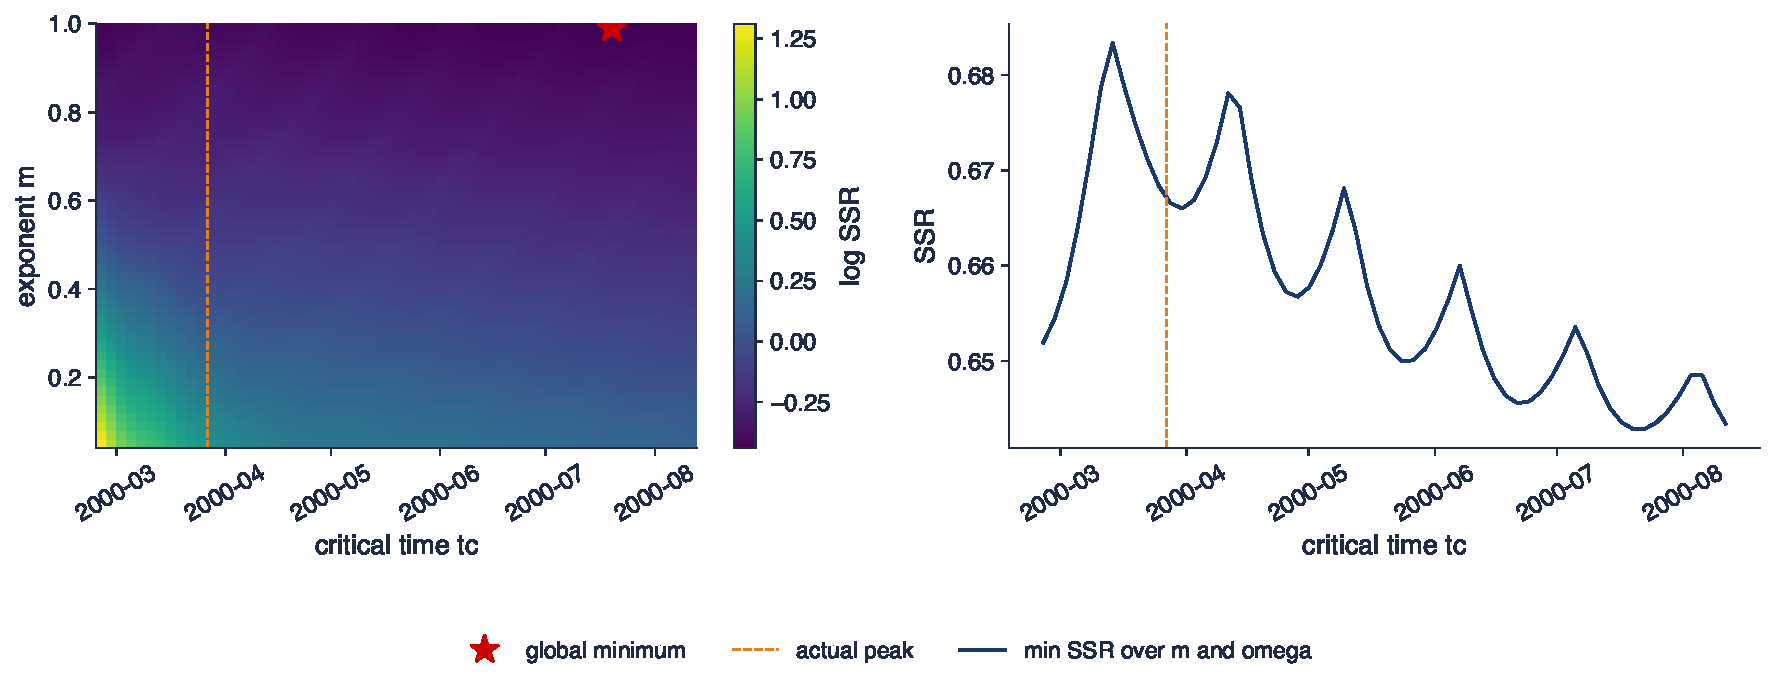
\includegraphics[width=0.97\textwidth,height=0.56\textheight,keepaspectratio]{tsa_ch13_cost.pdf}
\end{center}
\vspace{-0.25cm}
\begin{itemize}
    \item Nasdaq 100, fereastra de la minimul din octombrie 1998 pînă la 30 de zile înainte de maximum; stînga: $\log \mathrm{SSR}$ după $(t_c, m)$, minimizat după $\omega \in [2, 25]$ (135\,360 de puncte de grilă, cu pasul liniar rezolvat în fiecare punct); dreapta: minimul după $m$ și $\omega$, ca funcție de $t_c$
\end{itemize}
\quantlet{TSA\_ch13\_estimation}{\qlurl{TSA_ch13_estimation}}
\end{frame}

\begin{frame}{Interpretarea peisajului funcției de cost}
\itemsize{\small}
\begin{itemize}
    \item Profilul după $t_c$ are 5 minime locale: un optimizator pornit de la alt $t_c$ poate ajunge în altă vale
    \begin{itemize}
        \item valurile provin din termenul oscilant: mutarea lui $t_c$ mută faza ciclurilor
    \end{itemize}
    \item Peisajul este plat: cel mai prost și cel mai bun $t_c$ diferă cu doar 6{,}3\% în SSR
    \begin{itemize}
        \item minimul global este la $m$ aproape de 1 și $t_c$ = 19 iulie 2000, mult după maximul real: datele abia identifică $t_c$
    \end{itemize}
    \item Lecția: o singură ajustare LPPL nu este niciodată suficientă; avem nevoie de multe ferestre și de filtru (Secțiunea 5)
\end{itemize}
\end{frame}

\begin{frame}{Exemplu rezolvat: ajustarea pentru Shanghai la sfîrșitul ferestrei}
\itemsize{\footnotesize}
\begin{itemize}
    \item Shanghai Composite, fereastra 20 martie 2014 -- 13 mai 2015 (281 de zile); estimări: $t_c = 2015{,}428$ (6 iunie 2015), $m = 0{,}392$, $\omega = 5{,}50$
    \begin{itemize}
        \item pasul 1 dă $\hat A = 8{,}893$, $\hat B = -1{,}270$, $\hat C_1 = 0{,}020$, $\hat C_2 = 0{,}074$, deci $\hat C = 0{,}076$
    \end{itemize}
    \item La $t_2 = 2015{,}361$ (ani): $\tau = t_c - t_2 = 0{,}067$, $\tau^m = 0{,}347$, $\ln\tau = -2{,}702$
    \begin{itemize}
        \item $\cos(\omega\ln\tau) = -0{,}656$, $\sin(\omega\ln\tau) = -0{,}754$
        \item $\widehat{\ln P} = 8{,}893 + (-0{,}440) + (-0{,}024) = 8{,}429$; observat $\ln P = 8{,}384$
    \end{itemize}
    \item În niveluri: ajustat 4579 față de observat 4376, o eroare de 4{,}7\%; cei trei termeni sînt nivelul $A$, creșterea de tip lege de putere și oscilația
\end{itemize}
\end{frame}

\begin{frame}{Ajustări LPPL cu 30 de zile înainte de maximum}
\itemsize{\footnotesize}
\begin{center}
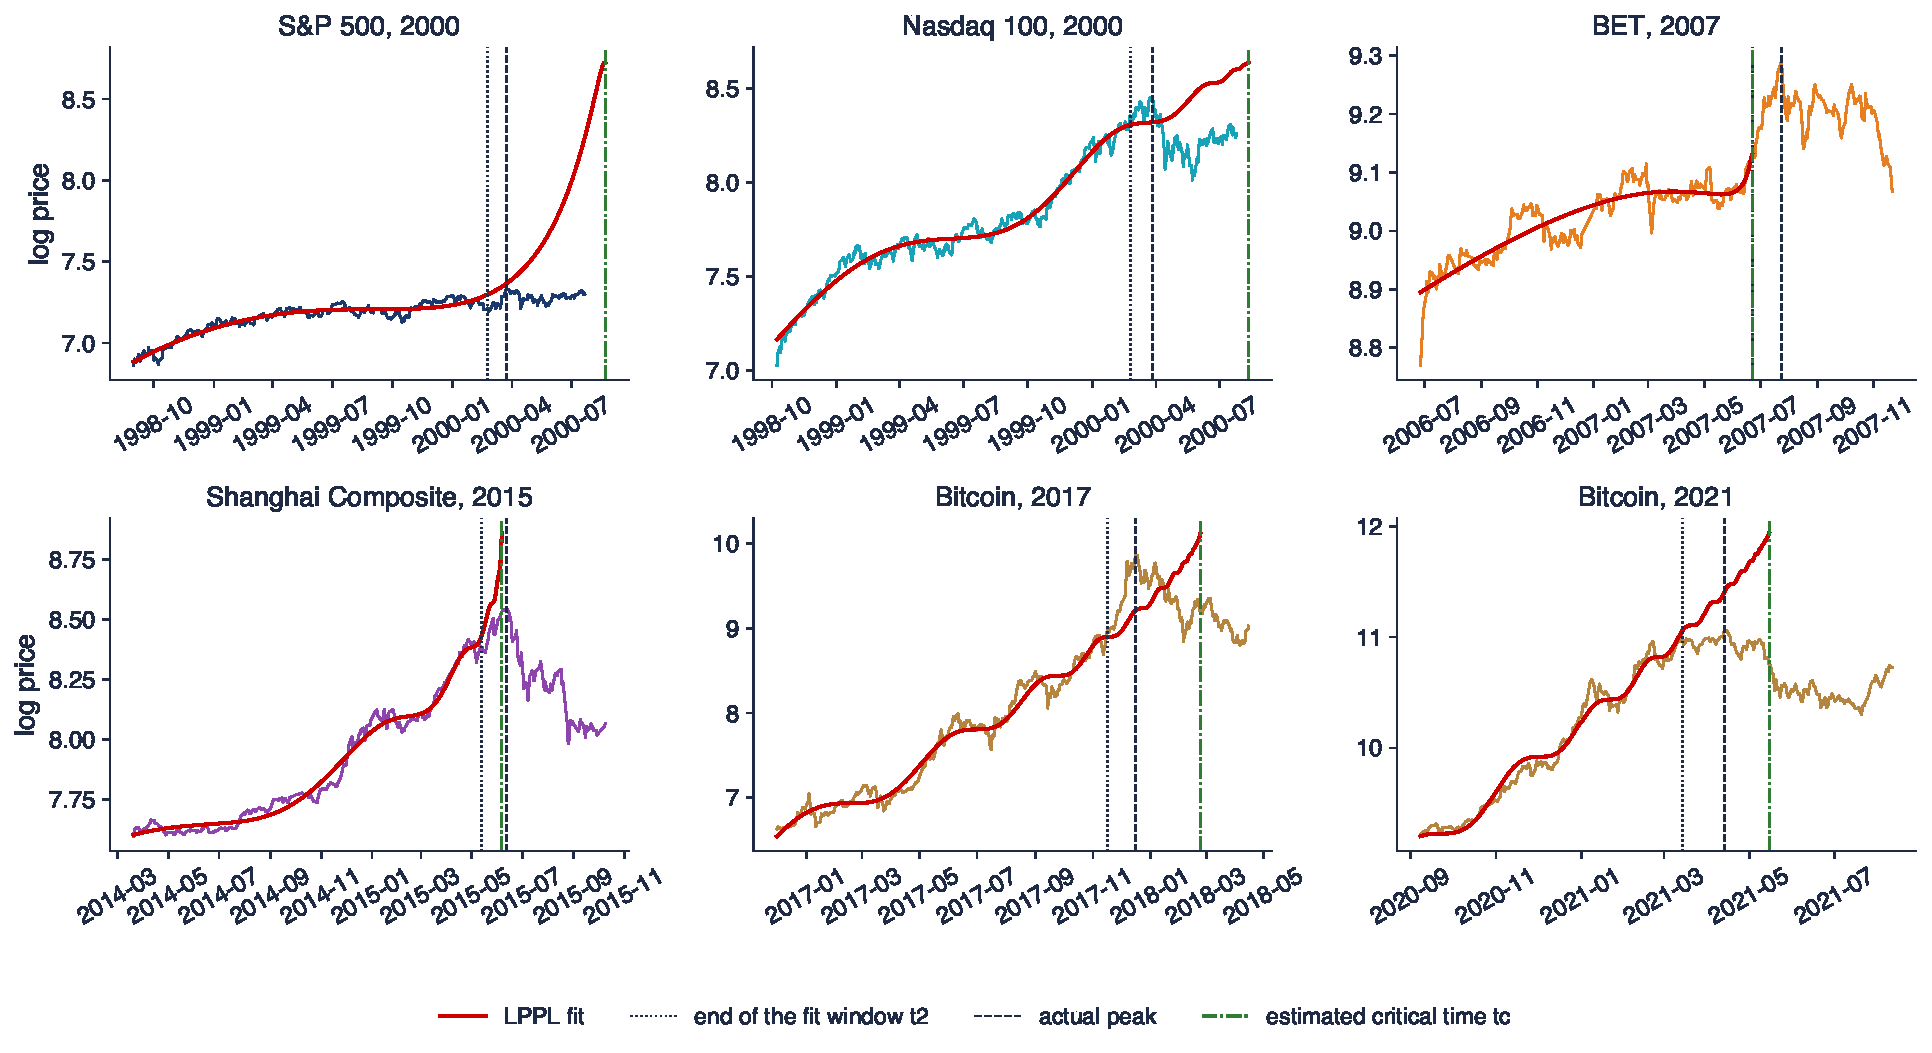
\includegraphics[width=0.97\textwidth,height=0.64\textheight,keepaspectratio]{tsa_ch13_fits.pdf}
\end{center}
\vspace{-0.25cm}
\begin{itemize}
    \item Fereastra: de la minimul dinaintea creșterii pînă la 30 de zile calendaristice înainte de maximum; traiectoria ajustată este prelungită pînă la $t_c$ estimat; datele de după fereastră sînt arătate doar pentru comparație
\end{itemize}
\quantlet{TSA\_ch13\_estimation}{\qlurl{TSA_ch13_estimation}}
\end{frame}

\begin{frame}{Interpretarea celor șase ajustări}
\itemsize{\footnotesize}
\begin{center}
\scriptsize
\begin{tabular}{lllrrrll}
\toprule
\textbf{Episodul} & $t_2$ & $\hat t_c$ & \textbf{Zile față de maxim} & $\hat m$ & $\hat\omega$ & \textbf{Param.} & \textbf{Toate} \\
\midrule
S\&P 500, 2000 & 23 februarie 2000 & 21 august 2000 & +150 & 1{,}00 & 1{,}0 & nu & nu \\
Nasdaq 100, 2000 & 25 februarie 2000 & 11 august 2000 & +137 & 1{,}00 & 5{,}9 & nu & nu \\
BET, 2007 & 22 iunie 2007 & 22 iunie 2007 & $-$32 & 0{,}69 & 1{,}0 & nu & nu \\
Shanghai Composite, 2015 & 13 mai 2015 & 6 iunie 2015 & $-$6 & 0{,}39 & 5{,}5 & da & da \\
Bitcoin, 2017 & 16 noiembrie 2017 & 22 februarie 2018 & +68 & 0{,}71 & 14{,}1 & nu & nu \\
Bitcoin, 2021 & 14 martie 2021 & 15 mai 2021 & +32 & 0{,}82 & 17{,}4 & nu & nu \\
\bottomrule
\end{tabular}
\end{center}
\begin{itemize}
    \item Zile față de maxim: $\hat t_c$ minus maximul real; Param.: ajustarea trece de condițiile asupra parametrilor; Toate: trece și de condițiile asupra reziduurilor
    \item Doar Shanghai trece de tot filtrul, cu $\hat t_c$ la mai puțin de o săptămînă de maximum; S\&P 500 și Nasdaq 100 ating limita $m = 1$: nicio creștere superexponențială în aceste ferestre
    \item Bitcoin nu trece de condiția erorii de 15\%: variațiile lui zilnice sînt prea mari pentru o singură traiectorie netedă
\end{itemize}
\end{frame}

\begin{frame}{Recapitulare: estimarea}
\itemsize{\small}
\begin{itemize}
    \item Patru parametri liniari prin OLS, trei neliniari ($t_c$, $m$, $\omega$) prin căutare: metoda \refFS
    \item Suprafața de cost este accidentată și plată după $t_c$: timpul critic este slab identificat
    \item O fereastră, o ajustare: doar unul dintre cele șase episoade dă o ajustare complet calificată cu 30 de zile înainte de maximum
\end{itemize}
\end{frame}


%=============================================================================
\section{Încrederea obținută din multe ferestre}
%=============================================================================

\begin{frame}{Indicatorul de încredere LPPLS}
\itemsize{\small}
\begin{itemize}
    \item Pînă acum $t_1$ a fost minimul dinaintea creșterii, o dată cunoscută doar \textbf{după} bulă; în timp real începutul nu este cunoscut
    \begin{itemize}
        \item remediul: pentru fiecare dată de sfîrșit $t_2$ (azi), ajustăm LPPL pe 29 de ferestre $[t_2 - L, t_2]$, $L = 750, 725, \dots, 50$ de zile de tranzacționare \refSZ
    \end{itemize}
    \item Indicatorul $=$ ponderea ferestrelor care se încheie la $t_2$ și au o ajustare calificată \refShanghai; 0: nicio fereastră nu vede o bulă, 1: toate văd
    \begin{itemize}
        \item LPPLS (singularitatea LPPL) este numele folosit pentru acest indicator; ecuația este aceeași
    \end{itemize}
    \item Două versiuni în acest capitol
    \begin{itemize}
        \item \textbf{condițiile asupra parametrilor}: $B$, $m$, $\omega$, $t_c$, oscilații, amortizare
        \item \textbf{toate condițiile}: și eroarea de 15\%, testul Lomb și reziduurile staționare (\refSZ)
    \end{itemize}
    \item Se calculează doar cu date pînă la $t_2$: un indicator în timp real; o alarmă cînd depășește un prag fixat dinainte (aici 0,2)
\end{itemize}
\end{frame}

\begin{frame}{Multe ferestre, o singură dată de sfîrșit}
\itemsize{\footnotesize}
\begin{center}
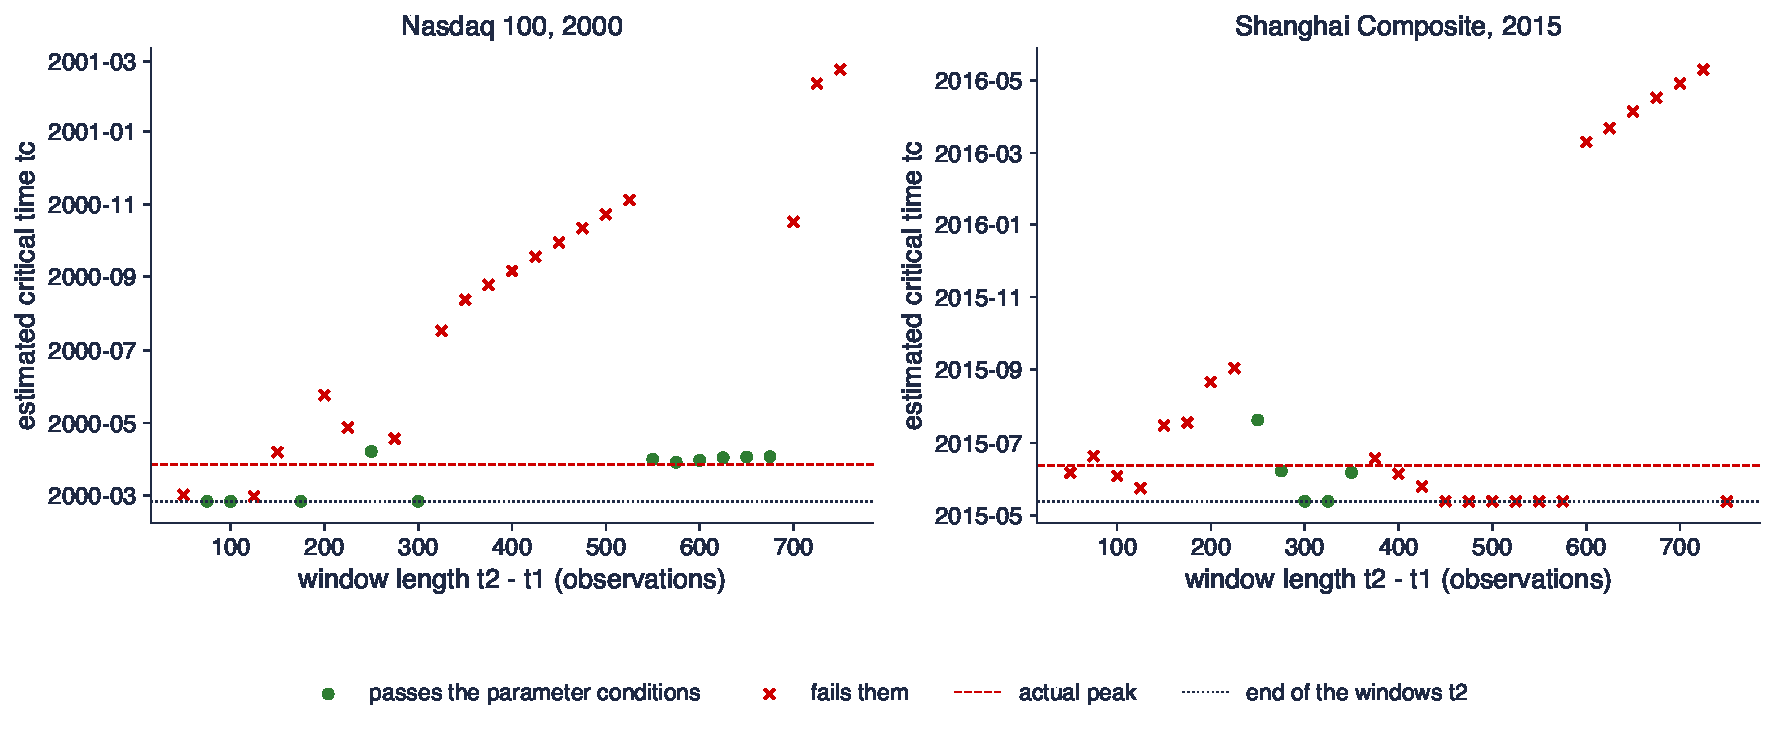
\includegraphics[width=0.97\textwidth,height=0.6\textheight,keepaspectratio]{tsa_ch13_windows.pdf}
\end{center}
\vspace{-0.25cm}
\begin{itemize}
    \item $t_c$ estimat pentru fiecare dintre cele 29 de ferestre care se încheie cu 30 de zile înainte de maximum; puncte verzi: ajustarea trece de condițiile asupra parametrilor; cruci roșii: nu trece
\end{itemize}
\quantlet{TSA\_ch13\_confidence}{\qlurl{TSA_ch13_confidence}}
\end{frame}

\begin{frame}{Interpretarea ferestrelor}
\itemsize{\small}
\begin{itemize}
    \item Nasdaq 100 (sfîrșit 25 februarie 2000): 11 din 29 de ferestre trec de condițiile asupra parametrilor, 1 de tot filtrul
    \begin{itemize}
        \item $\hat t_c$ calificat: mediana 30 martie 2000, intervalul 10\%--90\% 25 februarie 2000 -- 2 aprilie 2000; maximul real 27 martie 2000
    \end{itemize}
    \item Shanghai (sfîrșit 13 mai 2015): 5 din 29 trec de condițiile asupra parametrilor; mediana $\hat t_c$ 6 iunie 2015, maximul real 12 iunie 2015
    \begin{itemize}
        \item condiția asupra lui $m$ cade cel mai des: doar 41\% dintre ferestrele Shanghai au $0{,}01 \le m \le 0{,}99$
    \end{itemize}
    \item Ferestrele scurte pun $t_c$ imediat după $t_2$; ferestrele lungi îl împrăștie: lungimea ferestrei este o alegere de modelare ascunsă
\end{itemize}
\end{frame}

\begin{frame}{Indicatorul în jurul a patru maxime}
\itemsize{\footnotesize}
\begin{center}
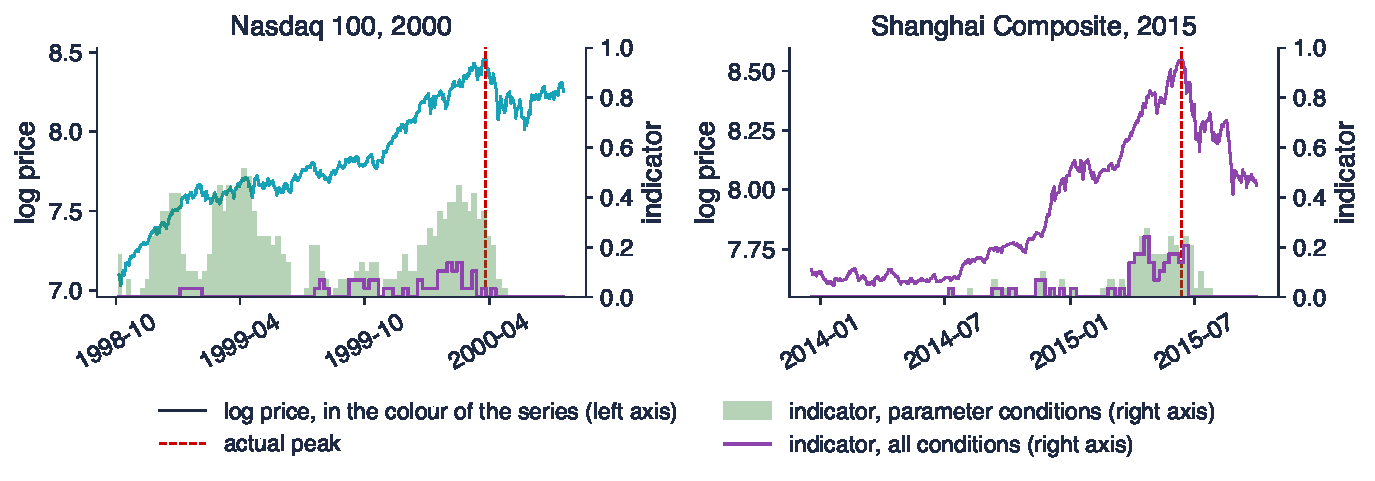
\includegraphics[width=0.97\textwidth,height=0.64\textheight,keepaspectratio]{tsa_ch13_ci.pdf}
\end{center}
\vspace{-0.25cm}
\begin{itemize}
    \item Prețul logaritmic (axa din stînga) și indicatorul (axa din dreapta) la fiecare 5 zile de tranzacționare (Bitcoin: 7 zile), de la 18 luni înainte pînă la 4 luni după maximum; zona verde: condițiile asupra parametrilor; linia mov: toate condițiile
\end{itemize}
\quantlet{TSA\_ch13\_confidence}{\qlurl{TSA_ch13_confidence}}
\end{frame}

\begin{frame}{Interpretarea indicatorului}
\itemsize{\small}
\begin{itemize}
    \item Nasdaq 100: versiunea pe parametri atinge 0{,}52 la 7 aprilie 1999, cu un an înainte de maximum, și crește din nou în ultimele luni; versiunea completă rămîne sub 0{,}14
    \begin{itemize}
        \item Shanghai: ambele versiuni cresc în cele două luni dinaintea maximului (maximum 0{,}24 la 22 aprilie 2015)
    \end{itemize}
    \item BET: cel mai puternic semnal cu filtrul complet, 0{,}28, vine la 28 august 2007, după maximum: ajustările descriu atunci ultima parte a creșterii, nu viitorul
    \begin{itemize}
        \item Bitcoin 2017: versiunea pe parametri ajunge la 0{,}66 la 29 decembrie 2017; versiunea completă este aproape mereu 0 (condiția erorii de 15\%)
    \end{itemize}
    \item Indicatorul se aprinde în bule, dar devreme, tîrziu și cu întreruperi; alegerea filtrului schimbă imaginea
\end{itemize}
\end{frame}

\begin{frame}{Timpul critic se mută odată cu datele}
\itemsize{\footnotesize}
\begin{center}
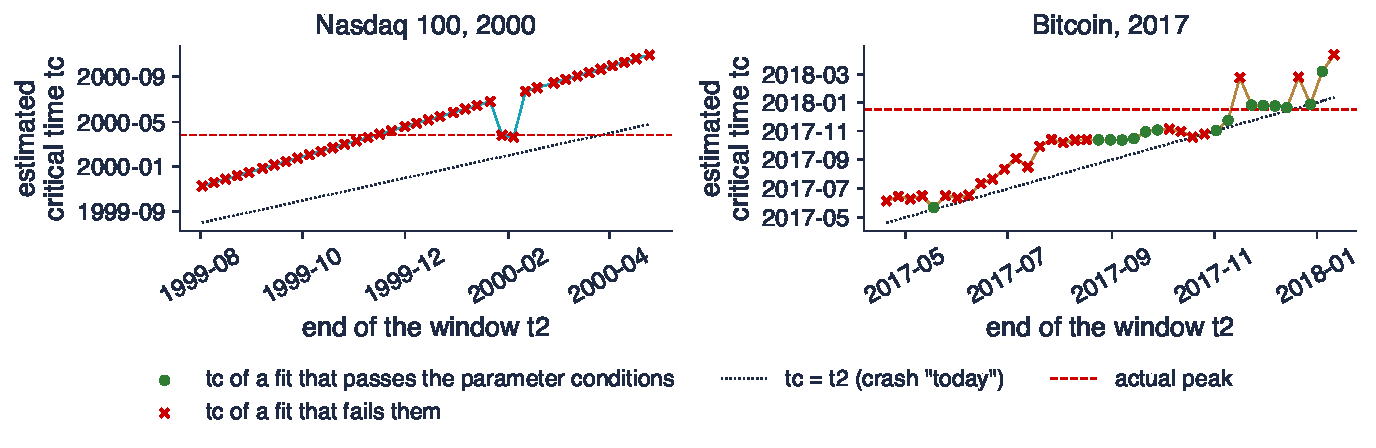
\includegraphics[width=0.97\textwidth,height=0.6\textheight,keepaspectratio]{tsa_ch13_tc_path.pdf}
\end{center}
\vspace{-0.25cm}
\begin{itemize}
    \item Începutul ferestrei fixat la minimul dinaintea creșterii; sfîrșitul $t_2$ se mută de la 8 luni înainte pînă la o lună după maximum (săptămînal); fiecare punct: $\hat t_c$ al ajustării care se încheie la $t_2$
\end{itemize}
\quantlet{TSA\_ch13\_confidence}{\qlurl{TSA_ch13_confidence}}
\end{frame}

\begin{frame}{Interpretarea timpului critic care se mută}
\itemsize{\small}
\begin{itemize}
    \item Nasdaq 100: pe 38 de date de sfîrșit, $\hat t_c$ variază de la 9 noiembrie 1999 la 30 octombrie 2000 (356 de zile); niciuna dintre aceste ajustări nu trece de condițiile asupra parametrilor
    \begin{itemize}
        \item Bitcoin 2017: intervalul 21 mai 2017 -- 12 aprilie 2018; 38\% dintre ajustări trec; eroarea mediană 65 de zile
    \end{itemize}
    \item Multe puncte stau aproape de dreapta $t_c = t_2$: ajustarea spune adesea „sfîrșitul este acum”, săptămînă după săptămînă
    \begin{itemize}
        \item o prognoză care se tot mută odată cu datele este o descriere a trecutului, nu o predicție
    \end{itemize}
    \item Alegerea, după crah, a singurei ferestre al cărei $\hat t_c$ a fost corect înseamnă \textbf{look-ahead bias} (folosirea informației din viitor)
\end{itemize}
\end{frame}

\begin{frame}{Recapitulare: încrederea obținută din multe ferestre}
\itemsize{\small}
\begin{itemize}
    \item Începutul unei bule nu este cunoscut: ajustăm 29 de ferestre pentru fiecare dată de sfîrșit
    \item Indicatorul = ponderea ferestrelor calificate; depinde puternic de filtru
    \item $\hat t_c$ se mută odată cu sfîrșitul datelor: raportați dispersia lui pe ferestre, niciodată o singură valoare
\end{itemize}
\end{frame}


%=============================================================================
\section{O evaluare onestă a prognozei crahurilor}
%=============================================================================

\begin{frame}{Capcane în evaluarea prognozelor de crah}
\itemsize{\small}
\begin{itemize}
    \item \textbf{Look-ahead bias}: folosirea informației de după $t_2$
    \begin{itemize}
        \item alegerea lui $t_1$ la minimul creșterii, a episoadelor după crah sau a filtrului după ce am văzut rezultatele
    \end{itemize}
    \item \textbf{Selecția}: studierea doar a bulelor care s-au spart; creșterile care nu s-au încheiat cu un crah sînt uitate
    \item \textbf{Alarmele false și frecvențele de bază}: o alarmă este utilă doar dacă un crah este \textbf{mai probabil după o alarmă} decît într-o zi obișnuită
    \begin{itemize}
        \item comparația: $P(\text{crah} \mid \text{alarmă})$ față de $P(\text{crah})$, frecvența necondiționată
    \end{itemize}
    \item Un test corect fixează totul dinainte (ferestre, filtru, prag, definiția crahului) și rulează pe tot eșantionul
\end{itemize}
\end{frame}

\begin{frame}{Alarmele pe tot eșantionul}
\itemsize{\footnotesize}
\begin{center}
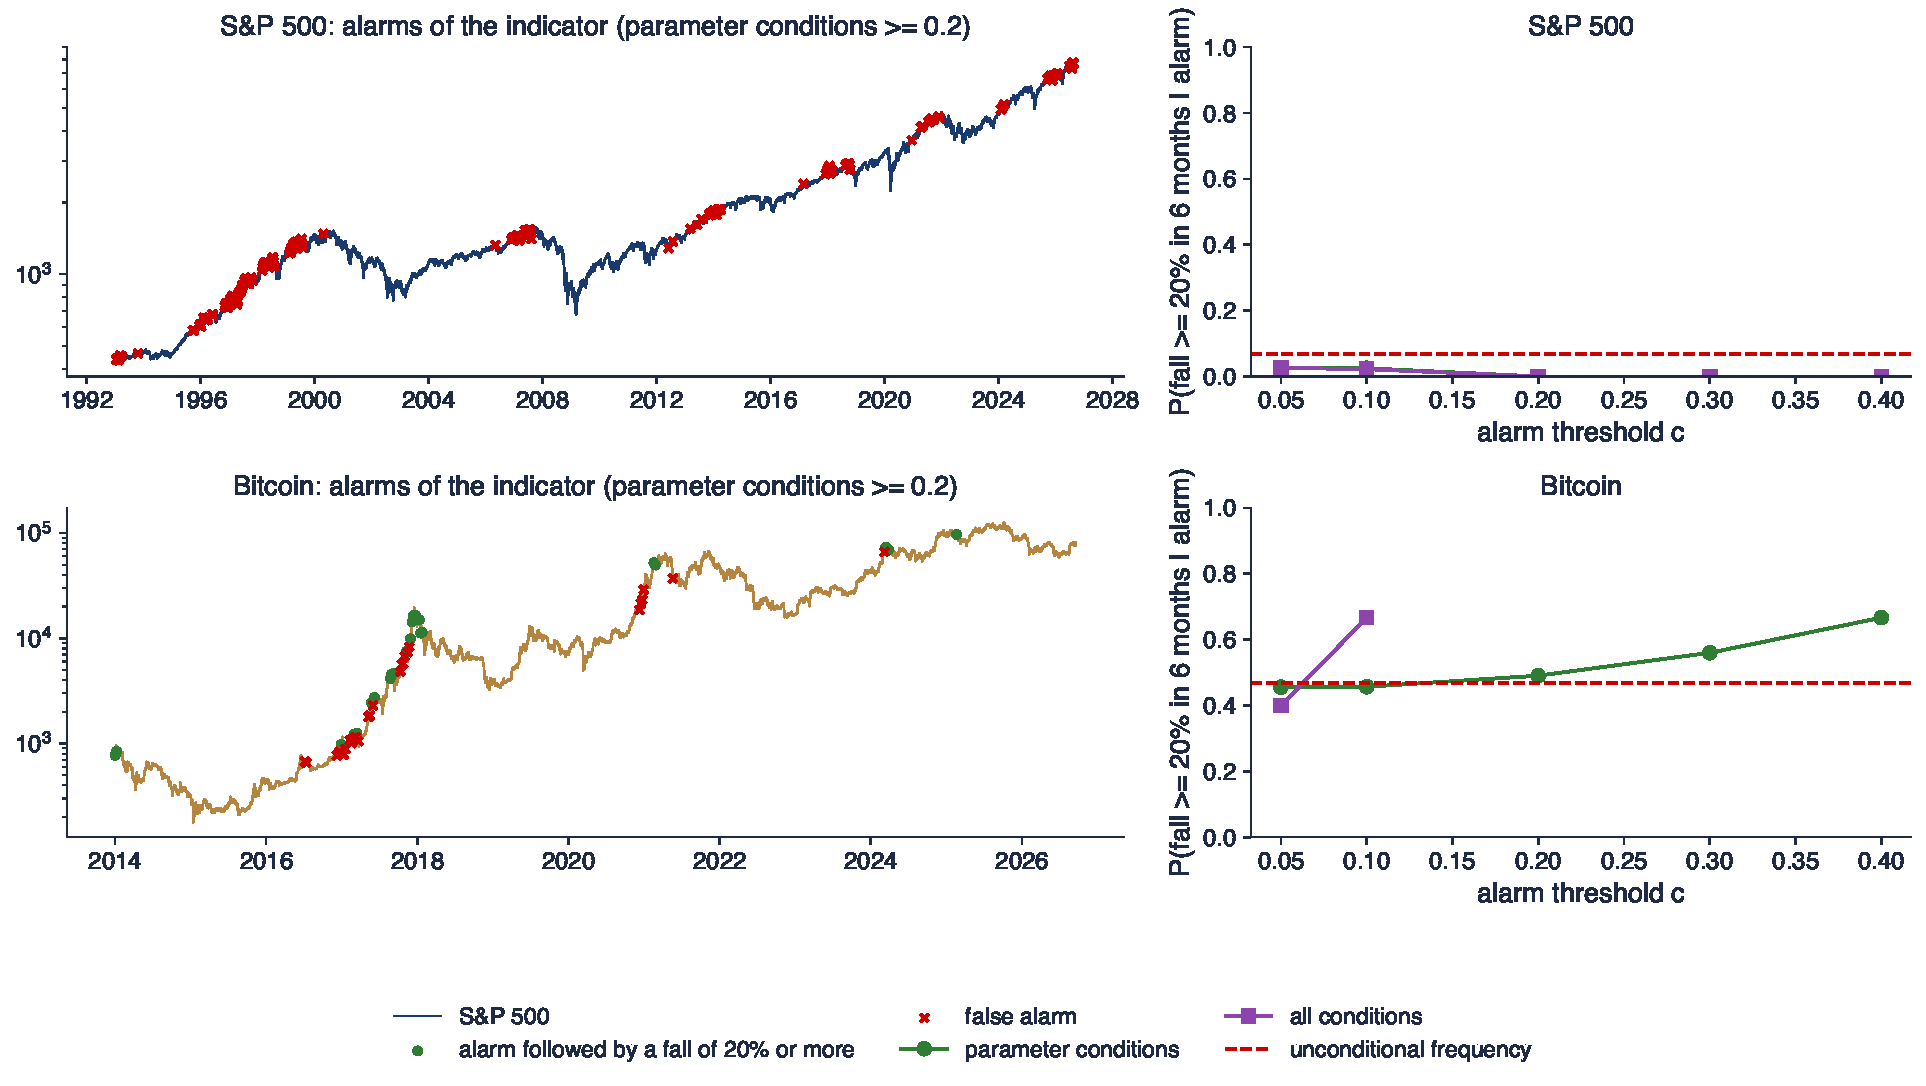
\includegraphics[width=0.97\textwidth,height=0.62\textheight,keepaspectratio]{tsa_ch13_eval.pdf}
\end{center}
\vspace{-0.25cm}
\begin{itemize}
    \item Indicatorul la fiecare 5 zile de tranzacționare (S\&P 500, ianuarie 1993 -- septembrie 2026) și la fiecare 7 zile (Bitcoin, ianuarie 2014 -- septembrie 2026); un crah: o scădere de cel puțin 20\% în cele 182 de zile de după alarmă; dreapta: rata de reușită în funcție de prag
\end{itemize}
\quantlet{TSA\_ch13\_evaluation}{\qlurl{TSA_ch13_evaluation}}
\end{frame}

\begin{frame}{Interpretarea evaluării}
\itemsize{\small}
\begin{itemize}
    \item S\&P 500: o scădere de 20\% în șase luni urmează după 7\% dintre toate datele, dar după 0\% dintre datele cu alarmă (pragul 0,2, condițiile asupra parametrilor)
    \begin{itemize}
        \item 20 de grupuri de alarme, niciunul urmat de o astfel de scădere în șase luni; alarmele apar în creșteri calme și constante
        \item dintre cele 4 scăderi de 20\% sau mai mult din ianuarie 1993, 2 au avut o alarmă în cele șase luni dinaintea maximului (2007 și 2022), dar scăderile au venit mai tîrziu
    \end{itemize}
    \item Bitcoin: frecvența de bază 47\%, după o alarmă 49\%: aproape niciun cîștig; 12 dintre cele 14 scăderi de 20\% au avut o alarmă înainte de maximum
    \begin{itemize}
        \item scăderile de 20\% sînt atît de frecvente la Bitcoin încît aproape orice alarmă pare „corectă”; pragurile mai mari ajută puțin, pe foarte puține date (56\% la 0,3, pe 4\% dintre date)
    \end{itemize}
    \item Indicatorul spune „aceasta seamănă cu un regim de bulă”, nu „crahul vine în următoarele șase luni”
\end{itemize}
\end{frame}

\begin{frame}{Literatura despre prognoza crahurilor}
\itemsize{\small}
\begin{itemize}
    \item Reușite raportate de autorii metodei
    \begin{itemize}
        \item \refJiang: bulele chinezești din 2007 și 2009 diagnosticate dinainte; \refShanghai: maximul Shanghai din 2015 anunțat înainte să aibă loc
        \item \refGerlach: bulele Bitcoin din 2012--2018 analizate cu indicatorul de încredere
    \end{itemize}
    \item Evaluări critice
    \begin{itemize}
        \item \refFeig: termenul log-periodic adaugă puțin odată ce se ține cont de eroarea de estimare
        \item \refBJ: pe multe crahuri, condițiile LPPL sînt rareori toate îndeplinite înainte de crah; parametrii sînt instabili
    \end{itemize}
    \item Propriile noastre cifre arată același lucru: indicatorul reacționează la creșterile puternice, dar momentul lui este imprecis și alarmele lui sînt adesea false
\end{itemize}
\end{frame}

\begin{frame}{Posibilitățile și limitele modelului LPPL}
\itemsize{\small}
\begin{itemize}
    \item \textbf{Poate}: descrie o creștere cu ritm accelerat și corecții tot mai scurte prin cîțiva parametri interpretabili
    \begin{itemize}
        \item măsura cît de mult seamănă azi o piață cu o bulă, pe multe ferestre (indicatorul)
    \end{itemize}
    \item \textbf{Nu poate}: da data unui crah; $t_c$ este sfîrșitul regimului, iar regimul se poate încheia cu o scădere lentă
    \begin{itemize}
        \item nici să ne spună dacă prețul este peste valoarea fundamentală: pentru asta sînt necesare fundamentele
    \end{itemize}
    \item Folosiți-l împreună cu testele de rădăcini explozive, cu fundamentele (rapoarte de evaluare) și cu măsuri de risc precum VaR 1\% (\tsachlink{https://danpele.github.io/Time-Series-Analysis/RO/Cursuri/capitol5_volatilitate_conditionata_garch.pdf}{Capitolul 5}), nu singur
\end{itemize}
\end{frame}

\begin{frame}{Recapitulare: o evaluare onestă}
\itemsize{\small}
\begin{itemize}
    \item Fixați ferestrele, filtrul, pragul și definiția crahului înainte de a vă uita la rezultate
    \item Comparați rata de reușită după alarme cu frecvența de bază; numărați alarmele false
    \item LPPL descrie bine bulele; ca instrument de datare a crahurilor, rezultatele lui sînt slabe
\end{itemize}
\end{frame}


%=============================================================================
\section{Contribuția posibilă a AI}
%=============================================================================

\begin{frame}{Contribuția posibilă a AI}
\itemsize{\small}
\begin{itemize}
    \item \textbf{Cod}: o primă versiune a recursiei BSADF, a ajustării în doi pași Filimonov--Sornette, a indicatorului pe multe ferestre
    \item \textbf{Explicații}: o a doua explicație a argumentului ratei de hazard sau a log-periodicității, cu cifrele dumneavoastră
    \item \textbf{Explorare}: indicatorul pe multe piețe și perioade, cu filtre diferite, după un protocol fixat dinainte
    \item Exemplu de prompt
    \begin{itemize}
        \item \aiprompt{Write Python code that fits the LPPL model to the daily log price of the Shanghai Composite between two dates with the Filimonov-Sornette method (OLS for A, B, C1, C2; grid search plus Nelder-Mead for tc, m, omega), checks the filter conditions of Shu and Zhu (2020) and plots the fit.}
    \end{itemize}
\end{itemize}
\end{frame}

\begin{frame}{Verificări necesare}
\itemsize{\small}
\begin{itemize}
    \item Simulați o traiectorie LPPL cu parametri cunoscuți plus zgomot și verificați că codul regăsește $t_c$, $m$ și $\omega$
    \item Convențiile de semn: $B < 0$ pentru o bulă în creștere; testul de rădăcini explozive folosește coada din dreapta, nu coada din stînga din \tsachlink{https://danpele.github.io/Time-Series-Analysis/RO/Cursuri/capitol3_radacini_unitare_modele_arima.pdf}{Capitolul 3}
    \item Valorile critice: SADF și GSADF au nevoie de propriile valori critice simulate, nu de tabelul Dickey--Fuller
    \item Fără look-ahead: orice mărime la data $t_2$ trebuie să folosească doar date pînă la $t_2$
    \item Un crah „prezis” de un răspuns AI după ce a avut loc nu este o predicție; cereți lista completă a alarmelor și a alarmelor false
    \item Fiecare referință citată: trebuie să existe; verificați DOI-ul
\end{itemize}
\end{frame}


%=============================================================================
\section{Rezumat}
%=============================================================================

\begin{frame}{Idei de reținut}
\itemsize{\small}
\begin{itemize}
    \item O bulă este un preț peste valoarea fundamentală; o bulă rațională trebuie să crească exploziv
    \item Testele ADF la dreapta (SADF, GSADF, BSADF) detectează și datează episoadele explozive cu datele disponibile la fiecare dată
    \item LPPL: creștere superexponențială cu oscilații log-periodice, care se încheie la un timp critic $t_c$
    \item Estimați în doi pași (OLS + căutare după $t_c$, $m$, $\omega$), filtrați ajustările, folosiți multe ferestre
    \item Judecați prognozele prin rata de reușită față de frecvența de bază, cu toate alarmele false: datarea crahurilor rămîne dificilă
\end{itemize}
\end{frame}

\begin{frame}{Formule de reținut}
\itemsize{\small}
{\renewcommand{\arraystretch}{1.35}\begin{center}
\scriptsize
\begin{tabular}{ll}
\toprule
\textbf{Mărimea} & \textbf{Formula} \\
\midrule
Bulă rațională & $P_t = F_t + B_t$, \quad $E_t[B_{t+1}] = (1+r)B_t$ \\
ADF la dreapta & $\Delta y_t = a + \delta y_{t-1} + \varepsilon_t$, \quad $H_1$: $\delta > 0$ \\
GSADF, BSADF & $\sup_{r_2}\sup_{r_1}\mathrm{ADF}_{r_1}^{r_2}$, \quad $\mathrm{BSADF}(r_2) = \sup_{r_1}\mathrm{ADF}_{r_1}^{r_2}$, \quad $r_0 = 0{,}01 + 1{,}8/\sqrt T$ \\
LPPL & $\ln P(t) = A + B(t_c - t)^m + C(t_c - t)^m\cos(\omega\ln(t_c - t) - \phi)$ \\
Forma liniară & $\ln P(t) = A + Bf_t + C_1g_t + C_2h_t$, \quad $C = \sqrt{C_1^2 + C_2^2}$ \\
Raportul de scală & $\lambda = e^{2\pi/\omega}$ \\
Amortizarea & $m|B|/(\omega|C|) \ge 1$ \\
Indicatorul & ponderea ferestrelor calificate care se încheie la $t_2$ \\
\bottomrule
\end{tabular}
\end{center}
}
\end{frame}

\begin{frame}{Autoevaluare (1/2)}
\itemsize{\small}
\begin{itemize}
    \item \textbf{Întrebare}: într-o bulă Blanchard--Watson cu $r = 1\%$ și $\pi = 0{,}95$, cu cît crește bula într-o perioadă în care supraviețuiește?
    \begin{itemize}
        \item \textbf{Răspuns}: cu $1{,}01/0{,}95 - 1 \approx 6{,}3\%$; durata medie de viață $1/(1 - 0{,}95) = 20$ de perioade
    \end{itemize}
    \item \textbf{Întrebare}: un ADF la dreapta pe o fereastră dă $\hat\delta = 0{,}004$ cu SE 0,002. Este fereastra explozivă la 5\%, dacă valoarea critică este 1,5?
    \begin{itemize}
        \item \textbf{Răspuns}: da: $t = 0{,}004/0{,}002 = 2 > 1{,}5$; respingem rădăcina unitară în favoarea unei rădăcini explozive
    \end{itemize}
    \item \textbf{Întrebare}: de ce folosim coada din dreapta și nu coada din stînga din \tsachlink{https://danpele.github.io/Time-Series-Analysis/RO/Cursuri/capitol3_radacini_unitare_modele_arima.pdf}{Capitolul 3}?
    \begin{itemize}
        \item \textbf{Răspuns}: alternativa este $\rho > 1$ (exploziv), nu $\rho < 1$ (staționar); dovada pentru ea este un $t$ pozitiv mare
    \end{itemize}
\end{itemize}
\end{frame}

\begin{frame}{Autoevaluare (2/2)}
\itemsize{\small}
\begin{itemize}
    \item \textbf{Întrebare}: o ajustare LPPL dă $\omega = 6{,}28$. Cu ce factor se micșorează timpul rămas pînă la $t_c$ între două corecții?
    \begin{itemize}
        \item \textbf{Răspuns}: $\lambda = e^{2\pi/6{,}28} \approx e \approx 2{,}72$
    \end{itemize}
    \item \textbf{Întrebare}: o ajustare are $m = 1{,}0$, la marginea spațiului de căutare. Este o ajustare calificată de bulă?
    \begin{itemize}
        \item \textbf{Răspuns}: nu: filtrul cere $m \le 0{,}99$; $m = 1$ este un trend liniar în $t$, nu unul accelerat
    \end{itemize}
    \item \textbf{Întrebare}: un indicator dă alarme înainte de 8 din 10 crahuri. Este un predictor bun?
    \begin{itemize}
        \item \textbf{Răspuns}: încă nu: avem nevoie și de alarmele false și de frecvența de bază; dacă alarmele apar aproape în fiecare zi, este ușor să prinzi 8 crahuri
    \end{itemize}
\end{itemize}
\end{frame}

\begin{frame}{Idee de proiect}
\itemsize{\small}
\begin{itemize}
    \item \textbf{Este BET azi într-o bulă?} Un protocol în timp real, fixat înainte de a vedea rezultatul
    \begin{itemize}
        \item BSADF pe BET și BET-TR săptămînal; indicatorul din acest capitol pe BET zilnic
        \item evaluarea din Secțiunea 6 pe BET din 2000: alarme, alarme false, frecvența de bază
    \end{itemize}
    \item Extensii
    \begin{itemize}
        \item raportul preț--profit în locul prețului; Bitcoin și Ethereum împreună
        \item comparați cu modelele cu schimbare de regim din \tsachlink{https://danpele.github.io/Time-Series-Analysis/RO/Cursuri/capitol10_spatiul_starilor_kalman_markov_switching.pdf}{Capitolul 10}
    \end{itemize}
    \item Lecturi suplimentare despre Bursa de Valori București: \refPeleCrash
    \item Urmează: \tsachlink{https://danpele.github.io/Time-Series-Analysis/RO/Cursuri/capitol14_modele_garch_multivariate.pdf}{Capitolul 14}, modele GARCH multivariate
\end{itemize}
\end{frame}


%=============================================================================
\section{Bibliografie}
%=============================================================================

\begin{frame}{Bibliografie (1/2)}
\itemsize{\tiny}
\begin{itemize}
    \item Blanchard, O. J., \& Watson, M. W. (1982). Bubbles, rational expectations and financial markets. NBER Working Paper 945. \href{https://doi.org/10.3386/w0945}{doi:10.3386/w0945}
    \item Brée, D. S., \& Joseph, N. L. (2013). Testing for financial crashes using the log periodic power law model. \textit{International Review of Financial Analysis}, 30, 287--297. \href{https://doi.org/10.1016/j.irfa.2013.05.005}{doi:10.1016/j.irfa.2013.05.005}
    \item Dickey, D. A., \& Fuller, W. A. (1979). Distribution of the estimators for autoregressive time series with a unit root. \textit{Journal of the American Statistical Association}, 74(366), 427--431. \href{https://doi.org/10.1080/01621459.1979.10482531}{doi:10.1080/01621459.1979.10482531}
    \item Fama, E. F. (2014). Two pillars of asset pricing. \textit{American Economic Review}, 104(6), 1467--1485. \href{https://doi.org/10.1257/aer.104.6.1467}{doi:10.1257/aer.104.6.1467}
    \item Feigenbaum, J. A. (2001). A statistical analysis of log-periodic precursors to financial crashes. \textit{Quantitative Finance}, 1(3), 346--360. \href{https://doi.org/10.1088/1469-7688/1/3/306}{doi:10.1088/1469-7688/1/3/306}
    \item Filimonov, V., \& Sornette, D. (2013). A stable and robust calibration scheme of the log-periodic power law model. \textit{Physica A}, 392(17), 3698--3707. \href{https://doi.org/10.1016/j.physa.2013.04.012}{doi:10.1016/j.physa.2013.04.012}
    \item Garber, P. M. (1990). Famous first bubbles. \textit{Journal of Economic Perspectives}, 4(2), 35--54. \href{https://doi.org/10.1257/jep.4.2.35}{doi:10.1257/jep.4.2.35}
    \item Gerlach, J.-C., Demos, G., \& Sornette, D. (2019). Dissection of Bitcoin\textquoteright s multiscale bubble history from January 2012 to February 2018. \textit{Royal Society Open Science}, 6(7), 180643. \href{https://doi.org/10.1098/rsos.180643}{doi:10.1098/rsos.180643}
    \item Greenwood, R., Shleifer, A., \& You, Y. (2019). Bubbles for Fama. \textit{Journal of Financial Economics}, 131(1), 20--43. \href{https://doi.org/10.1016/j.jfineco.2018.09.002}{doi:10.1016/j.jfineco.2018.09.002}
    \item Huang, C., \& Petukhina, A. (2022). \textit{Applied Time Series Analysis and Forecasting with Python}. Springer. \href{https://doi.org/10.1007/978-3-031-13584-2}{doi:10.1007/978-3-031-13584-2}
    \item Jiang, Z.-Q., Zhou, W.-X., Sornette, D., Woodard, R., Bastiaensen, K., \& Cauwels, P. (2010). Bubble diagnosis and prediction of the 2005--2007 and 2008--2009 Chinese stock market bubbles. \textit{Journal of Economic Behavior \& Organization}, 74(3), 149--162. \href{https://doi.org/10.1016/j.jebo.2010.02.007}{doi:10.1016/j.jebo.2010.02.007}
    \item Johansen, A., Ledoit, O., \& Sornette, D. (2000). Crashes as critical points. \textit{International Journal of Theoretical and Applied Finance}, 3(2), 219--255. \href{https://doi.org/10.1142/S0219024900000115}{doi:10.1142/S0219024900000115}
    \item Kindleberger, C. P., \& Aliber, R. Z. (2005). \textit{Manias, Panics and Crashes: A History of Financial Crises} (5th ed.). Palgrave Macmillan. \href{https://doi.org/10.1057/9780230628045}{doi:10.1057/9780230628045}
    \item Lomb, N. R. (1976). Least-squares frequency analysis of unequally spaced data. \textit{Astrophysics and Space Science}, 39(2), 447--462. \href{https://doi.org/10.1007/BF00648343}{doi:10.1007/BF00648343}
    \item Pele, D. T., \& Mazurencu-Marinescu, M. (2012). Modelling stock market crashes: The case of Bucharest Stock Exchange. \textit{Procedia -- Social and Behavioral Sciences}, 58, 533--542. \href{https://doi.org/10.1016/j.sbspro.2012.09.1030}{doi:10.1016/j.sbspro.2012.09.1030}
    \item Phillips, P. C. B., \& Shi, S. (2020). Real time monitoring of asset markets: Bubbles and crises. In \textit{Handbook of Statistics: Financial, Macro and Micro Econometrics Using R}, 61--80. Elsevier. \href{https://doi.org/10.1016/bs.host.2018.12.002}{doi:10.1016/bs.host.2018.12.002}
\end{itemize}
\end{frame}

\begin{frame}{Bibliografie (2/2)}
\itemsize{\tiny}
\begin{itemize}
    \item Phillips, P. C. B., Shi, S., \& Yu, J. (2015a). Testing for multiple bubbles: Historical episodes of exuberance and collapse in the S\&P 500. \textit{International Economic Review}, 56(4), 1043--1078. \href{https://doi.org/10.1111/iere.12132}{doi:10.1111/iere.12132}
    \item Phillips, P. C. B., Shi, S., \& Yu, J. (2015b). Testing for multiple bubbles: Limit theory of real-time detectors. \textit{International Economic Review}, 56(4), 1079--1134. \href{https://doi.org/10.1111/iere.12131}{doi:10.1111/iere.12131}
    \item Phillips, P. C. B., Wu, Y., \& Yu, J. (2011). Explosive behavior in the 1990s Nasdaq: When did exuberance escalate asset values? \textit{International Economic Review}, 52(1), 201--226. \href{https://doi.org/10.1111/j.1468-2354.2010.00625.x}{doi:10.1111/j.1468-2354.2010.00625.x}
    \item Shiller, R. J. (2015). \textit{Irrational Exuberance} (3rd ed.). Princeton University Press. \href{https://doi.org/10.1515/9781400865536}{doi:10.1515/9781400865536}
    \item Shu, M., \& Zhu, W. (2020). Detection of Chinese stock market bubbles with LPPLS confidence indicator. \textit{Physica A}, 557, 124892. \href{https://doi.org/10.1016/j.physa.2020.124892}{doi:10.1016/j.physa.2020.124892}
    \item Sornette, D. (2017). \textit{Why Stock Markets Crash: Critical Events in Complex Financial Systems}. Princeton University Press. \href{https://doi.org/10.23943/princeton/9780691175959.001.0001}{doi:10.23943/princeton/9780691175959.001.0001}
    \item Sornette, D., Demos, G., Zhang, Q., Cauwels, P., \& Zhang, Q. (2015). Real-time prediction and post-mortem analysis of the Shanghai 2015 stock market bubble and crash. \textit{Journal of Investment Strategies}, 4(4), 77--95. \href{https://doi.org/10.21314/JOIS.2015.063}{doi:10.21314/JOIS.2015.063}
    \item Sornette, D., Johansen, A., \& Bouchaud, J.-P. (1996). Stock market crashes, precursors and replicas. \textit{Journal de Physique I}, 6(1), 167--175. \href{https://doi.org/10.1051/jp1:1996135}{doi:10.1051/jp1:1996135}
\end{itemize}
\end{frame}

\end{document}
